\documentclass[english, 10pt, letterpaper]{article}
\usepackage[letterpaper, margin=0.8in]{geometry}
\usepackage[utf8]{inputenc}

\title{The origin, distribution, and genetic interactions of \emph{KRAS} alleles across cancer types}
\author{
    Joshua H. Cook\textsuperscript{1,2,3,7},
    Giorgio E. M. Melloni\textsuperscript{3,7}, 
    Doga C. Gulhan\textsuperscript{3}, 
    Peter J. Park\textsuperscript{3,4{*}}, 
    Kevin M. Haigis\textsuperscript{1,2,5,6{*}}
}

\usepackage[T1]{fontenc}
\usepackage{babel}
\usepackage{amsmath}
\usepackage{amssymb}
\usepackage{graphicx}
\usepackage{fancyhdr}
\pagestyle{fancy}
\fancyhf{}
\renewcommand{\headrulewidth}{0pt}
\setlength{\headheight}{0pt}

% Supplementary figure numbering.
\newcommand{\beginsupplement}{%
        \setcounter{table}{0}
        \renewcommand{\thetable}{\arabic{table}}%
        \setcounter{figure}{0}
        \renewcommand{\thefigure}{\arabic{figure}}%
    }

% Single spaces after periods.
\frenchspacing

% Page numbering.
\pagenumbering{arabic}
\rfoot{\thepage}

% Font to Helvetica.
\usepackage{helvet}
\renewcommand{\familydefault}{\sfdefault}

% Specific command for the KRAS gene.
\newcommand{\KRAS}{\emph{KRAS}}
% Specific command for the KRAS protein.
\newcommand{\kras}{K-RAS}

% Spacing between lines
\linespread{2.0}

\begin{document}

%%TC:ignore

\maketitle

\thispagestyle{fancy}

1. Department of Cancer Biology, Dana Farber Cancer Institute, Boston, Massachusetts.
2. Department of Medicine, Brigham \& Women’s Hospital, Harvard Medical School, Boston, Massachusetts.
3. Department of Medical Informatics, Harvard Medical School, Boston, Massachusetts, USA.
4. Ludwig Center at Harvard, Boston, MA 02115, USA.
5. Broad Institute, Cambridge, Massachusetts, USA.
6. Harvard Digestive Disease Center, Harvard Medical School, Boston, Massachusetts.
7. These authors contributed equally.

{*}corresponding authors:
\newline{} \hspace*{1cm} Kevin M. Haigis (kevin\_haigis@dfci.harvard.edu)
\newline{} \hspace*{1cm} Peter J. Park (peter\_park@hms.harvard.edu)

\newpage
\section*{}
% Keep within 100-150 words.
Mutational activation of \KRAS{} promotes the initiation and progression of cancers, especially in the colorectum, pancreas, lung, and blood plasma, with varying prevalence of specific activating missense mutations. 
Although epidemiological studies connect specific alleles to clinical outcomes, the mechanisms underlying the distinct clinical characteristics of mutant \KRAS{} alleles are unclear. 
Here, we analyzed 13,492 samples from these four tumor types to examine allele- and tissue-specific genetic properties associated with oncogenic \KRAS{} mutations. 
The prevalence of known mutagenic mechanisms partially explained the observed spectrum of \KRAS{} activating mutations, but the prevalence of most alleles across the different cancers could not be explained in this way, suggesting that biological selection underlies the tissue-specific frequencies of mutant alleles. 
Consistent with experimental studies that have identified distinct signaling properties associated with each mutant form of \kras{}, a genetic analysis revealed that each \KRAS{} allele was associated with a distinct and tissue-specific comutation network. 
Moreover, we identified genetic dependencies associated with specific mutant \KRAS{} alleles. 
Overall, this analysis demonstrates that the genetic interactions associated with oncogenic \KRAS{} mutations are allele- and tissue-specific, underscoring the complexity that drives their clinical behaviors. 
\newpage
%%TC:endignore

\section*{}

Located at a critical signaling junction between extracellular growth receptors and pro-growth pathways, \KRAS{} is one of the most commonly mutated genes in cancer \cite{Simanshu2017, Bailey2018}.
However, it is only found frequently mutated in a few cancers, with the highest frequencies in colorectal adenocarcinoma (COAD), lung adenocarcinoma (LUAD), multiple myeloma (MM), and pancreatic adenocarcinoma (PAAD).
Importantly, the mutations found in \KRAS{} vary substantially across cancers, pointing to significant differences in signaling behavior of the alleles that complement the environment of the specific cellular context \cite{Haigis2017, Poulin2019}.

When mutated at one of its four hotspot codons, 12, 13, 61, and 146, \KRAS{} is thought to hyperactivate many downstream effector pathways, for instance, the MAPK and PI3K-Akt signaling pathways \cite{Simanshu2017}.
Previous studies have documented substantial differences in the biochemistry and signaling properties of the common \kras{} variants (extensively reviewed by \cite{Miller2012, Li2018}).
\kras{} operates as a molecular switch, activating downstream pathways when GTP-bound, but inactive when GDP-bound following the hydrolysis of the $\gamma$-phosphate.
This reaction is catalyzed by GTPase-activating proteins (GAPs) and the exchange of the GDP for a new GTP is facilitated by guanine nucleotide exchange factors (GEFs) \cite{Barbacid1987}.
Activating \KRAS{} mutations result in elevated downstream pathway activation by increasing the steady-state concentration of GTP-bound \kras{}.
More specifically, mutations to codons 12, 13, and 61 reduce the rate of intrinsic and/or GAP-mediated hydrolysis, and mutants at 13 and 61, but not 12, also enhance the rate of nucleotide exchange \cite{Hunter2015a, Smith2013}.
Alternatively, 146 mutations do not alter the rate of GTP hydrolysis, but cause hyperactivation through an increased rate of GDP exchange \cite{Feig1988RelationshipProteins., Edkins2006, Janakiraman2010, Poulin2019}.
Additional biochemical, structural, and signaling distinctions have been identified between different mutant alleles at the same amino acid position \cite{Li2018, Hunter2015a, Poulin2019, Hobbs2019AtypicalCancer., Yu2018, Kovalski2019, Ihle2012, Spoerner2004, Smith2014a, Pantsar2018}.

Likely as a consequence of their distinct properties, associations have been uncovered between the specific \KRAS{} mutation status of a patient's cancer and its drug-response or clinical outcome \cite{Haigis2017, Li2018}.
For instance, a retrospective meta-analysis suggested that COAD tumors with a \KRAS{} G13D allele are sensitive to anti-EGFR therapies, a treatment generally discouraged for \KRAS{}-mutant tumors \cite{DeRoock2010}. 
It has recently been proposed, via computational and experimental means, that differential interaction kinetics between \kras{} G13D and the Ras GAP NF-1 explain this effect \cite{McFall2019, Rabara2019, Zafra2019}.
Another example is that the \KRAS{} G12D allele is associated with reduced overall survival in advanced PAAD when separately compared to patients with WT \KRAS{}, \KRAS{} G12R, or \KRAS{} G12V \cite{Bournet2016}.
Thus far, the hypothesis has been that the different biological properties of the mutant \KRAS{} alleles is the cause of these clinical distinctions.
However, it is also possible that allele-specific genetic interactions drive the varying clinical outcomes.

For the reasons noted above, understanding the heterogeneous properties of the \KRAS{} alleles is essential to effectively treating \KRAS{}-driven cancers.
The prominent reductionist strategy of treating all \KRAS{} mutants the same has so far proven insufficient.
Thus, the current study describes genetic interactions found in tumors with the common \KRAS{} alleles in COAD, LUAD, MM, and PAAD.
The origins of \KRAS{} mutations were studied to assess the extent to which latent mutational processes determined the allelic distribution.
Further, comutation networks were constructed for each \KRAS{} allele and interrogated to identify properties of the alleles.
Finally, allele-specific genetic dependencies were analyzed to identify potential therapeutic targets.
Integrating these two forms of genetic interactions highlighted the distinct effects of each \KRAS{} allele on the genetic landscape, and thus behavior, of the tumor.
We believe that an allele-specific and tissue-specific analysis such as this is necessary to fully understand the nature of the most potent oncogenes.



\section*{Results}

\subsection*{\KRAS{} alleles are non-uniformly distributed across cancers.}

This study utilized publicly available sequencing data of COAD, LUAD, MM, and PAAD.
There were whole exome or genome data available for 1,536 COAD (including 256 hypermutated samples), 891 LUAD, 1,201 MM, and 1,395 PAAD samples.
In addition, there were targeted-sequencing data available for 3,329 COAD (including 464 hypermutated samples), 4,160 LUAD, 61 MM, and 919 PAAD samples.
More information on the data is available in the Methods and Supplementary Tables 1 and 2.

\KRAS{} was most frequently mutated by single nucleotide substitutions at one of four "hotspots": codons 12, 13, 61, and 146. (Fig. \ref{fig:mutational-signatures-main}a; Supplementary Table 3).
Glycine 12 and 13 can be transformed to six different amino acids (A, C, D, R, S, and V) through single nucleotide changes in the first two guanine residues.
Glutamine 61 can be mutated to six other amino acids (E, H, K, L, P, and R) and a stop codon via a single nucleotide mutation.
Alanine 146 can become one of six other amino acids (E, G, P, S, T, and V) from mutations to a single nucleotide.

Of these hotspots, codon 12 mutations accounted for 81.7\% of all mutations followed by codon 13 (8.4\%), 61 (7.3\%) and 146 (2.5\%).
Adjusting for the different yearly incidence of each cancer, the distribution of mutations was 76.8\%, 11.4\%, 8.1\%, and 3.7\% at codons 12, 13, 61, and 146, respectively.
PAAD had the greatest frequency of \KRAS{} mutations at 86.3\%, followed by COAD (41.4\%), LUAD (35.3\%), and MM (21.9\%) (Fig. \ref{fig:mutational-signatures-main}b).
Further, there was substantial variability of the alleles found at these hotspots across the four \KRAS{}-driven cancers (Fig. \ref{fig:mutational-signatures-main}a). 
Notably, the most variation in \KRAS{} alleles was found in MM, and it was the only cancer where a non-G12 allele was the most frequent.
At codon 12, LUAD had an enrichment for G12C mutations.
COAD had a unique enrichment of G13D and A146T alleles, while PAAD was distinct in its high frequency of G12R mutations.


\subsection*{The \KRAS{} alleles have different mutagenic origins.}

One explanation for the distinct allelic frequencies across cancer types is that tissue-specific mutational processes determine the distribution.
To explore this hypothesis, the active mutational processes in the tumor samples were elucidated using mutational signatures \cite{Alexandrov2013} (Supplementary Tables 4 and 5; the signature numbers refer to those in the catalog \cite{Alexandrov2020TheCancer.}). 
Briefly, all single-nucleotide mutations can be represented by the combination of the six possible pyrimidine to purine base substitutions (C>T, C>A, C>G, T>A, T>C, T>G) and all possible 3’ and 5’ flanking bases. 
This composes a mutational spectrum with 96 possible trinucleotide contexts. 
The signatures comprising this spectrum were discovered in whole exome and whole genome sequencing data using non-negative matrix factorization and measured in each sample using non-negative least squares regression (see Methods; Supplementary Fig. \ref{sfig:mutational-signatures-supp}).

As expected, the distribution of the levels of each mutational signature were highly variable across tumor types.
The most common signatures in COAD, MM, and PAAD, were the "clock-like" single base substitution (SBS) signatures SBS1 and SBS5, which are believed to accumulate with age \cite{Alexandrov2015}. 
LUAD was enriched for a mutational signature of exogenous cause, tobacco smoke carcinogens (SBS4). 
Within each cancer type, the relative abundance of the mutational signatures were generally uniform, regardless of the \KRAS{} allele (Fig. \ref{fig:mutational-signatures-main}c). 
An exception was for microsatellite instable (MSI) tumors, in which defective DNA mismatch repair and other related signatures dominated (Supplementary Fig. \ref{sfig:mutational-signatures-supp}a and b).
Thus, for each cancer, the allelic frequency of \KRAS{} was not primarily caused by differential activity of mutational processes in individual tumors.

However, each mutational process is not equally likely to cause each \KRAS{} allele.
The probability that the allele for an individual tumor was caused by any detectable mutational process was calculated using the trinucleotide context of the \KRAS{} mutation and the relative activity of the mutational signature in that tumor (Fig. \ref{fig:mutational-signatures-main}d).
In general, such probabilities reflected the underlying distribution of signatures, as seen in the similarities between Figures \ref{fig:mutational-signatures-main}c and \ref{fig:mutational-signatures-main}d, suggesting that the specific set of mutational processes present in a tumor was highly influential in determining the eventual \KRAS{} mutation.

However, there were notable exceptions to this trend.
For example, in COAD and PAAD, SBS18 (navy blue bars), likely caused by damage from reactive oxygen species \cite{Viel2017, Pilati2017}, was strongly associated with G12C mutations (Fig. \ref{fig:mutational-signatures-main}d).
This corroborated the previous finding that \KRAS{} G12C mutations were more frequent in patients with MUTYH-Associated Polyposis \cite{Viel2017}, an autosomal recessive disease form of COAD caused by biallelic loss-of-function mutations to the gene encoding the DNA glycosylase, \emph{MUTYH}, responsible for clearing 8-oxoguanine:A mismatches that can cause the G12C mutation.
In LUAD, the \KRAS{} G12A/C/V mutations were primarily attributable to mutations caused by tobacco smoke, whereas \KRAS{} G12D mutations were most likely attributable to clock-like mutations (Fig. \ref{fig:mutational-signatures-main}d).
In MM, SBS9, associated with mutations introduced by polymerase $\eta$ repair of activation-induced deaminase (AID) activity \cite{Alexandrov2013, Rogozin2018DNACancer., Petljak2016UnderstandingCancer.}, was strongly linked with Q61H (Fig. \ref{fig:mutational-signatures-main}c, d), the most common \KRAS{} mutation in that cancer.
Finally, SBS8, of unknown etiology, had a substantial probability of causing some of the \KRAS{} alleles, particularly G12V, across all four cancers.
SBS17, also of uncertain etiology though linked to oxidative stress in other cancers \cite{Tomkova2018MutationalAsymmetry}, was the main cause for Q61H mutations in PAAD.


\subsection*{The frequency of most \KRAS{} alleles cannot be solely attributed to the prevalence of detected mutagens.}

The extent to which mutational signatures represent the mechanism driving \KRAS{} allelic diversity was further analyzed by calculating the predicted frequency of each allele in each tumor sample based on the frequency of mutations in the same trinucleotide context throughout the genome (Fig. \ref{fig:obs-vs-pred-main}; Supplementary Table 6).
The null hypothesis tested was that, assuming the cancer would acquire a \KRAS{} mutation, any one of the common alleles (found in greater than 3\% of the tumor samples for a given cancer) was sufficient, and thus, the frequency of the \KRAS{} alleles would be determined by the mutational processes alone.
The average predicted frequencies across the samples of each cancer were compared against the observed allele frequencies.
The alleles below the diagonal line were predicted to be more frequent than observed, while those above the line were more frequently observed than predicted.
In COAD, G13D was predicted to be the most frequent allele.
G12D/V mutations were considerably underestimated (Chi-squared test, p < 0.05, triangles); inversely, the frequencies of G12S and A146T mutations were significantly overestimated in COAD (Chi-squared test, p < 0.05, triangles).
In LUAD, the frequencies of the G12A/D/V alleles were predicted quite accurately, though the frequency of the most common allele, G12C, was substantially underestimated.
The high frequency of this allele has been attributed to its association with SBS4 caused by tobacco smoke (Fig. \ref{fig:mutational-signatures-main}c, d), but this result suggests there is additional biological pressure promoting this mutation in LUAD.
The frequencies of the \KRAS{} alleles were best predicted in MM, with an exception for the most frequent allele, Q61H, which was dramatically underestimated with a predicted frequency of 15.0\% but actual frequency of 35.7\% of \KRAS{} mutations.
In PAAD, all of the alleles were observed at a significantly different frequency than predicted by mutational signatures.

The correlations between the observed and predicted allele frequencies for each cancer were low, indicating that the frequencies of the \KRAS{} alleles were not strictly determined by the prevalence of their respective causative single nucleotide substitutions.
PAAD had the strongest concordance between the predicted and observed allele frequencies with a Pearson correlation coefficient of 0.75, while the other three cancers had coefficients around 0.50.
Interestingly, the codon 12 mutations demonstrated greater agreement between the observed and predicted frequencies in COAD, LUAD, and PAAD with correlation coefficients of 0.82, 0.83, and 0.84, respectively.

In addition to estimating the distribution of the common \KRAS{} alleles for each cancer, a similar analysis was conducted considering all of the alleles found frequently in at least one of the cancer types (Supplementary Fig. \ref{sfig:obs-vs-pred-supp}; Supplementary Table 7).
The alleles never or rarely found in each cancer were predicted to occur at frequencies ranging from 1.5\% (for Q61L in PAAD) to 10.5\% (for Q61K in LUAD), indicating that these alleles are not rare because their causative mutations do not occur, but instead due to weak oncogenic fitness in the tissue.
For instance, the fact that \KRAS{} A146T is exceedingly rare in PAAD, though predicted to consist of 8.9\% of \KRAS{} mutations, agrees with the previous determination that forced expression of \KRAS{} A146T does not induce pancreatic intraepithelial neoplasia (PanIN) \cite{Poulin2019}.
Thus, while it is likely that the active mutational processes in a tissue contributed to which \KRAS{} mutation was gained, they were not completely deterministic.
Instead, the particular biological properties of the alleles drive their selection, warranting further investigation into their genetic interactions.


\subsection*{The \KRAS{} alleles have distinct comutation networks.}

We reasoned that if biological selection is driving \KRAS{} allele selection in cancer, then distinct functions of each mutant form of \kras{} would be reflected in cooperating genetic events. 
An increased frequency of comutation with another gene suggests a cooperative effect, whereas a reduced frequency of comutation (compared to random) suggests that the second event is functionally redundant or that it introduces an inhibitory effect.
The extreme of the latter effect is commonly known as "mutual exclusivity."
For instance, in COAD, \emph{APC} comutation enhances the effects of oncogenic \KRAS{}-induced hyperactivation of the Wnt signaling pathway, essential for the growth of cancer stem cells in the intestinal crypts \cite{Janssen2006, Fearon2014, Sakai2018, Jauhri2017}.
Alternatively, in LUAD, the mutational activation of \emph{EGFR} was demonstrated to be cytotoxic in the presence of a \KRAS{} mutant, and, thus, the two are rarely found in the same tumor \cite{Unni2015EvidenceAdenocarcinoma., Ambrogio2017InAdenocarcinoma.}.

To this end, the comutation interactions between each \KRAS{} allele and every other mutated gene were investigated using a one-sided Fisher's exact test of association to identify increased rates of comutation and a test for mutual exclusivity proposed by Leiserson \emph{et al.} \cite{Leiserson2016} to identify reduced rates of comutation (compared to random; Supplementary Table 8).
The result of the comutation analysis on COAD tumors was a weakly connected network of the \KRAS{} alleles with only a few genes linking the alleles together (Fig. \ref{fig:comutation-main}a).
These linking genes tended to be well-studied cancer genes such as \emph{BRAF}, \emph{APC}, and \emph{TP53}.
Contrary to a common assumption, while \KRAS{} and \emph{TP53} are frequently found mutated in the same tumor, there is a detectable reduction in comutation between \emph{TP53} with \KRAS{} G12D and G13D compared to the rest of the alleles (Fig. \ref{fig:comutation-main}b).

Consistent with the idea that each allele is functionally distinct, a substantial number of genes comutated with just one \KRAS{} allele.
To gain functional insight into the network, genes known to physically interact with \kras{} \cite{Kovalski2019}, signal up- or downstream of \kras{} \cite{Kanehisa2017, Kanehisa2016KEGGAnnotation.}, or are known oncogenes \cite{Bamford2004TheWebsite., Sondka2018} were extracted (Fig. \ref{fig:comutation-main}b).
Several alleles had reduced comutation with \emph{NRAS} and \emph{BRAF} and increased comutation with \emph{APC} and \emph{PIK3CA}, interactions that have been previously documented \cite{Sensi2006MutuallyMelanoma., Jauhri2017, Seth2009ConcomitantCancer., Cisowski2016, Janssen2006, Sakai2018, Kennedy2011, Wang2013, Green2015, Yeang2008CombinatorialCancer., CancerGenomeAtlasNetwork2012}. 
Some novel interactions included increased comutation of \emph{PORCN} with \KRAS{} A146T, \emph{MTOR} with G12C, and \emph{SMAD4} with G12V.
Further, several of the alleles showed enrichment for cellular functions in their comutation networks (Fig. \ref{fig:comutation-main}c).
One of the strongest effects was an enrichment in the G12D comutation network of interactors with \emph{YWHAZ}, a 14-3-3 scaffolding protein implicated in modulating many interactions including the activity of Rho guanine nucleotide exchange factor 7 on RAC1 in phagocytosis and cell adhesion \cite{Angrand2006TransgenicSignaling.}.
Also, genes involved in the Hippo and Wnt signaling, key pathways in COAD, were enriched in the comutation networks of \KRAS{} G12V.
The comutation network of the G13D allele was enriched for genes implicated in apoptosis and senescence.
Additional genes of interest that had comutation interactions with \KRAS{} G12D are shown in Fig. \ref{fig:comutation-main}d and e.
These include increased comutation with \emph{AMER1}, a negative regulator of Wnt signaling \cite{Grohmann2007AMER1Membrane., Tanneberger2011StructuralAmer1.}

The \KRAS{} allele-specific comutation network uncovered in LUAD was far larger than that of COAD (Supplementary Fig. \ref{sfig:luad-comutation-network}).
This was likely caused by the higher mutation frequency in this cancer, increasing the statistical power to detect both increased and reduced comutation interactions.
As in the network derived from COAD, many of these genes were involved in integral \kras{} signaling pathways including an increased comutation interaction between \KRAS{} G12A and \emph{MAP2K3}, a reduced comutation interaction between \KRAS{} G12D and \emph{ERBB4} and a very strong increased rate of comutation between \KRAS{} G12C and \emph{STK11} (Supplementary Fig. \ref{sfig:luad-comutation-network}).
There were several intriguing cellular processes enriched in the LUAD networks for each allele (Fig. \ref{fig:comutation-main}c).
For example, \KRAS{} G12C had comutation interactions with many genes encoding proteins that interact with Myc ("PPI of MYC (TF)"), and the G12D comutation network was enriched with interactions with focal adhesion genes (Fig. \ref{fig:comutation-main}).

Conducting this analysis in MM was hampered by the fact that this cancer is known to be frequently multi-clonal.
As such, some detectable comutation events were mutations acquired by distinct populations in a single patient, potentially obfuscating true comutation interactions.
Due to this caveat, limiting the analysis to genes known to be recurrently mutated in MM reduced the chance of highlighting a false positive \cite{Sondka2018, Lohr2014WidespreadTherapy.}.
From this limited scope, it was discovered that \emph{NRAS} had reduced comutation with \KRAS{} G12D, Q61L, and Q61R, but one of the highest rates of comutation (18.5\%) with \KRAS{} Q61H, the most common \KRAS{} mutation in MM (Supplementary Fig. \ref{sfig:mm-comutation-heatmap}).
Interestingly, this was just below the rate of \emph{NRAS} mutation in \KRAS{} WT tumors (23.6\%), suggesting that the signaling of the Q61H allele is fundamentally different from the other \KRAS{} mutations in MM, especially G12D.

The \KRAS{} allele comutation network found in the PAAD tumor samples demonstrated that many genes had detectable comutation interactions with multiple alleles, primarily of reduced comutation (Supplementary Fig. \ref{sfig:paad-comutation-network}).
There were numerous genes that had opposing comutation interactions with different alleles.
Of these, four interact with or signal through \kras{} \cite{Kovalski2019, Kanehisa2017, Kanehisa2016KEGGAnnotation.} or are known oncogenes \cite{Bamford2004TheWebsite., Sondka2018}: \emph{TP53}, \emph{RNF43}, \emph{MAP2K4}, and \emph{RBM10} (Supplementary Fig. \ref{sfig:paad-comutation-network}).
Notably, while \emph{TP53} tended to comutate with \KRAS{} G12V, it was at a significantly lower rate than expected by random chance, given the overall mutation rate of \emph{TP53} and the mutational burden of the tumors.
There were many notable cellular functions and processes enriched in the comutation networks of the \KRAS{} alleles (Fig. \ref{fig:comutation-main}c) including the protein-protein interaction networks (PPIN) of SMAD1-3 and TGF-$\beta$ signaling.
While these SMAD gene sets were related, the underlying comutation interactions that drove the enrichment were different for each \KRAS{} allele (Fig. \ref{fig:comutation-main}f).
For instance, the comutation events of \emph{ACVR1B} with \KRAS{} were primarily with Q61H, whereas those with \emph{FLNA} were mostly with G12R.
These subtle differences suggest that specific and nuanced alterations of SMAD signaling best complement a given \KRAS{} allele in PAAD.


\subsection*{\KRAS{} allele-specific genetic dependencies reveal potential synthetic lethal vulnerabilities.}

The perturbations necessary to drive cancer expose vulnerabilities not present in the cell-of-origin.
For example, the microsatellite instability that often leads to cancer simultaneously makes the inhibition of Werner syndrome ATP-dependent helicase (WRN) lethal to the tumor cells \cite{Behan2019, Chan2019}.
As the \KRAS{} alleles have measurably different signaling behaviors and genetic interactions, they likely have specific genetic vulnerabilities.
To this end, data from a genome-wide, CRISPR-Cas9 knock-out screen of cancer cell lines \cite{Tsherniak2017, Meyers2017} were used to identify genes with \KRAS{} allele-specific genetic dependencies.
The analysis was restricted to \KRAS{} alleles for which there were at least 3 different cell lines with the mutation, limiting the following investigation to only COAD and PAAD cell lines.
Allele-specific enrichment for signaling pathways and cellular processes were identified using Gene Set Enrichment Analysis (GSEA), and individual genes demonstrating differential genetic dependency by \KRAS{} allele were identified using ANOVA and one-versus-rest t-tests.

For COAD, there were only a sufficient number of cell lines with WT \KRAS{} or G12D, G12V, and G13D mutations for this analysis.
Measuring for gene set enrichment revealed strong patterns in differential dependency of various cellular processes (Fig. \ref{fig:coad-dependency-main}a).
For example, genes involved in ERBB4 signaling tended to have a weaker lethal effect when knocked out in cell lines with \KRAS{} G12V mutations than in \KRAS{} G12D, G13D, or WT cell lines (Fig. \ref{fig:coad-dependency-main}b).
Similarly, the \KRAS{} G13D cell lines were less affected when genes involved in oxidative phosphorylation were targeted (Fig. \ref{fig:coad-dependency-main}c).
To discover individual genes with allele-specific interactions, each gene was tested for differential genetic dependency with the cell lines grouped by their \KRAS{} allele.
The resulting 62 genes were hierarchically clustered into 4 groups by their dependency scores (Figure \ref{fig:coad-dependency-main}d; Supplementary Table 9).
Genes in cluster 2 tended to have stronger genetic dependency in cell lines with \KRAS{} G12V, while those in cluster 3 demonstrated weaker dependency in G12D cell lines.
Four notable genes with allele-specific associations are displayed in Fig. \ref{fig:coad-dependency-main}e.
First, knocking-out \emph{LIN7C}, a gene that maintains the asymmetric distribution of membrane proteins in polarized epithelial cells \cite{Monastyrskaya2013MiR-199a-5pSyndrome}, had a more severe reduction on growth in \KRAS{} G13D cell lines compared to the others (Figure \ref{fig:coad-dependency-main}e).
Also, a regulator of apoptosis previously linked to dysregulated expression in cancer, \emph{TFPT}, demonstrated significantly greater dependency in G12D cell lines.
Interestingly, \emph{STARD9}, a gene encoding a kinesin required for mitotic spindle assembly \cite{Torres2011TheAssembly}, had moderate growth defects when knocked-out in all cell lines except those with a \KRAS{} G12D mutation.
Lastly, the kinetochore-associated protein (\emph{KNTC1}), a regulator of the mitotic checkpoint \cite{Chan2000HumanKinetochores., Scaerou2001TheKinetochore., Kops2005ZW10Kinetochore.}, which demonstrated moderate to strong lethal effects when knocked out in almost every cell line except for those with a \KRAS{} G12V allele (Figure \ref{fig:coad-dependency-main}e).

For the genetic dependency analysis of PAAD, the only \KRAS{} alleles with a sufficient number of cell lines were G12D, G12R, and G12V (there were not enough WT \KRAS{} cell lines to include in the analysis).
GSEA revealed substantial differences in the dependencies of critical cellular pathways (Supplementary Fig. \ref{sfig:paad-dependency-gsea}).
For instance, the G12D cell lines demonstrated a reduced dependency on the genes at the G2 and M DNA-damage checkpoint.
Moreover, the G12R cell lines were less dependent on PI3K signalling downstream of FGFR1, driven through a reduced dependency on \emph{FRS2} (fibroblast growth factor receptor substrate 2) and \emph{GRB2}, which encodes a protein linking EGFR to the GEF SOS1.
Similarly, the cell lines with \KRAS{} G12V mutations were less sensitive to the knock-out of genes implicated in cellular senescence.
This enrichment was driven by a significantly reduced dependence upon \emph{JUN}, which encodes the transcription factor c-JUN, and a beneficial impact on growth (a positive dependency score) from knocking-out \emph{MAPK8} (JNK-1), which regulates c-JUN via phosphorylation (Supplementary Fig. \ref{sfig:paad-dependency-heatmap}).
In these cell lines, 130 individual genes demonstrated \KRAS{} allele-specific genetic dependency (Supplementary Fig. \ref{sfig:paad-dependency-heatmap}; Supplementary Table 10).
Several noteworthy interactions include a regulator of cell cycle progression, \emph{KHDRBS1} \cite{Barlat1997ADomain}, the oxygen sensor, \emph{EGLN2} \cite{Ivan2017TheFeedbacks}, and a stabilizer of p53, \emph{BRI3BP} \cite{Ha2008HCCRBP-1Stabilization}.
Overall, the \KRAS{} alleles were associated with substantially different genetic dependencies on specific cellular processes, signaling pathways, and individual genes.


\subsection*{An integrated analysis of allele-specific comutation and genetic dependencies.}


The allele-specific comutation networks and the differential genetic dependency interactions were integrated to provide further insight into the distinctions between the \KRAS{} alleles.
Surprisingly, there was no overlap between the genes found to comutate with an allele and those with differential dependency.
This was likely due to the different biological pressures of the tumor microenvironment compared to the tissue culture used for the genetic dependency screens.
In addition, this suggests that the mutations obtained by genes with comutation interactions are not sufficiently modelled by a CRISPR-Cas9 knock-out, but are instead more complex alterations to the gene and encoded protein's behaviour.

(In progress.)





\section*{Discussion}

This study addresses the genetic complexity of cancer through a genetic interaction analysis of oncogenic \KRAS{} alleles in COAD, LUAD, MM, and PAAD. 
Measuring the levels of mutational signatures revealed that the cancer-specific distributions of \KRAS{} mutations were influenced, but not determined by, the active mutational processes in the tumor samples.
This result suggests that the biological properties of the \KRAS{} alleles, within the context of the tissue of origin, is an important factor in the positive selection of a \KRAS{} mutation during the evolution of a tumor.
To investigate these properties, we conducted statistical tests to determine patterns of comutating genes and genetic dependencies for each \KRAS{} allele in each cancer.
The former identified genes that comutated with specific \KRAS{} alleles at an unexpectedly high frequency, suggesting they were alterations that cooperated with the \KRAS{} allele to promote positive selection in the tumor.
Alternatively, some genes comutated with a \KRAS{} allele less frequently than expected by chance, suggesting they were functionally redundant mutations or introduced an inhibitory effect on the tumor's progression.
Finally, functional interactions were identified between \KRAS{} alleles and cellular processes and individual genes.
Together, these findings support a model in which the various oncogenic \KRAS{} mutations are not biologically redundant, but instead have distinct properties relevant to the treatment of \KRAS{} mutant tumors.

This analysis of \KRAS{} genetic networks in four different tumor types highlights the tissue-specific nature of genetic interactions. 
In places, we focused on the results from the analysis of COAD as it demonstrated a high variability in the types of \KRAS{} alleles, had limited exogenous mutational pressure (in contrast to the effects of smoking-induced mutations in LUAD), and we had a large number of WGS and WES data.
However, allele-specific genetic interactions were not consistent between tissues, demonstrating the complex relationship between the tissue-of-origin, \kras{} function, and cooperating genetic events.
While the intrinsic biochemical biochemical properties of a \kras{} mutant are maintained in each cancer, their downstream signaling properties, and ultimately their effects on tumorigenesis, are determined by basal configuration of the tissue-specific signaling network.

In addition to the importance of tissue-specificity, this study provides additional evidence that the study of oncogenes must be allele-specific.
We and others have repeatedly demonstrated the distinct effects of the \KRAS{} alleles, both computationally and experimentally, revealing many instances of substantial variation between different mutations of the same gene.
This is likely a more general principle applicable to many oncogenes, especially those with multiple mutational hotspots.


More broadly, this study has broad implications for the understanding of oncogene biology and for cancer therapy.
Whether a targeted therapy directly inhibits the activated oncoprotein or not, it is important to understand how allele-specific signaling properties and genetic interactions influence therapeutic response.
For instance, \emph{BRAF} activating mutations have been classified into three groups defined by their functional effects on the protein product \cite{Yao2015BRAFInhibition., Yao2017TumoursRAS.}, which consequently determines their response to different inhibitors \cite{Dagogo-Jack2019, Bracht2019BRAFRationale.}.
Moreover, the response of HER2 mutant cancers to HER2 inhibition varies depending on the tissue-of-origin of the cancer \cite{Hyman2018HERCancers}, which could be due to intrinsic signaling differences between the tissues-of-origin or to cooperating mutations unique to a specific cancer type. 
For cancer therapy to be truly precise, it will be key to appreciate and understand the complexity of the genetic networks in each cancer type.

%%TC:ignore



\section*{Methods}

\subsection*{Cancer sample data sources and acquisition}

Whole genome sequencing (WGS), whole exome sequencing (WES), and targeted gene panel sequencing ("targeted-sequencing") data were collected of colorectal adenocarcinoma (COAD), lung adenocarcinoma (LUAD), multiple myeloma (MM), and pancreatic adenocarcinoma (PAAD).
WES and WGS data were downloaded from cBioportal \cite{Gao2013, Cerami2012}, which included relevant projects from The Cancer Genome Atlas (TCGA) \cite{CancerGenomeAtlasNetwork2012, CancerGenomeAtlasResearchNetwork2014, CancerGenomeAtlasResearchNetwork.Electronicaddress:andrew_aguirredfci.harvard.edu2017} and other smaller studies. 
Additional data were acquired from the International Cancer Genome Consortium (ICGC) for pancreatic cancer \cite{Scarlett2011} and colorectal cancer. 
MM WES data were gathered from the Multiple Myeloma Research Foundation (MMRF)-CoMMpass online repository \cite{Walker2019AAnalysis.}.
Panel data for multiple cancers were retrieved from AACR Project Genomics Evidence Neoplasia Information Exchange (GENIE v5) \cite{AACRProjectGENIEConsortium2017AACRConsortium.}.
GENIE data are an aggregation of several different panels ranging from 30 to 600 genes.
\KRAS{} was included in all of the libraries. 
A detailed list of all cancer studies can be found in Supplementary Tables 1 and 2.


\subsection*{Hypermutated sample cutoff}

Some of the COAD samples had 5 to 10-times more mutations than the average, often due to microsatellite instability (MSI). 
A Gaussian mixed model was used to find the optimal cutoff based on available WGS and WES data. 
The top 17\% and 21\% of samples were considered hypermutants in WGS and WES, respectively.
The same 17\% cutoff was applied to the targeted-sequencing data. 
Hypermutants were not excluded from the identification of mutational signatures because signature 6 (marked as "MSI") is caused by MSI.


\subsection*{Tissue gene expression filter}

A conservative filter for tissue-specific gene expression was used to remove genes not expressed in the tissues of study. 
Normal tissue gene expression data was gathered from the GTEx Portal (12/03/2018) \cite{GTExConsortium2017} and The Human Protein Atlas (HPA, 12/03/2018) \cite{Uhlen2015, Uhlen2016}, and tumor expression data was collected from MMRF-CoMMpass (01/14/2019), TCGA-COAD, TCGA-LUAD, and TCGA-PAAD \cite{Walker2019AAnalysis., CancerGenomeAtlasNetwork2012, CancerGenomeAtlasResearchNetwork2014, CancerGenomeAtlasResearchNetwork.Electronicaddress:andrew_aguirredfci.harvard.edu2017}. 
A gene was considered “expressed” in a tissue if it met at least one of the following criteria: 1) a median expression level of at least 1 TPM across all samples of the tissue in GTEx, 2) indicated as expressed at at least 1 TPM in the HPA data set for the tissue, 3) expressed with a median level of 1 batch-normalized raw counts (using RSEM) in the corresponding tumor RNA-sequencing data.


\subsection*{Calculating overall distribution of hotspot mutations}
The frequency of mutations at the four hotspots of \KRAS{} across COAD, LUAD, MM, and PAAD was calculated by accounting for the different yearly incidence of each cancer type.
The incidence of cancers of the "colorectum," "lung and bronchus," "myeloma," and "pancreas" were obtained from the American Cancer Society \cite{Siegel2020Cancer2020.}: 3,870,000 colorectum, 5,930,000 lung and bronchus, 680,000 myeloma, 1,280,000 pancreas.
The incidences of COAD, LUAD, and PAAD were estimated by multiplying the number of cases of their respective tissue by the proportion they constitute: 95\%, 50\%, and 95\%, respectively \cite{Siegel2020Cancer2020., Meza2015Lung1973-2010.}.
The distribution of mutations to the hotspots across all cancers was calculated by finding the frequency within each cancer type, then combining those figures, weighting by their yearly incidence.


% \subsection*{Predicting effect of mutations on gene or protein function}

% The effect of a mutation on the function of a gene or encoded protein was predicted using SIFT \cite{Kumar2009, Vaser2016}, PolyPhen2 \cite{Adzhubei2010}, LRT \cite{Chun2009IdentificationGenomes.}, MutationTaster \cite{Schwarz2014MutationTaster2:Age.}, MutationAssessor \cite{Reva2007DeterminantsOptimization., Reva2011}, FATHMM \cite{Shihab2013}, MetaSVM \cite{Dong2015ComparisonStudies.}, and MetaLR \cite{Dong2015ComparisonStudies.}.
% Known clinically significant mutations were acquired from ClinVar \cite{Landrum2018ClinVar:Evidence.}.
% Annotations were applied using ANNOVAR \cite{Wang2010ANNOVAR:Data.}.
% A mutation was marked as deleterious if it was predicted as such by at least one of the prediction methods or declared as such by ClinVar.


\subsection*{Protein-Protein Interaction Network (PPIN)}

The PPIN used throughout the study was the combination of interactions from STRING \cite{VonMering2005, Szklarczyk2019}, HINT \cite{Das2012}, and BioPlex \cite{Huttlin2015}.


\subsection*{Identifying mutational signatures}

The genome-wide mutations of a sample can be deconvolved into mutational signatures that represent endogenous or exogenous mutagenic processes \cite{Alexandrov2013}. 
Single nucleotide variants (SNVs) from exomes or genomes were divided into 96 types, according to the 6 mutations of a pyrimidine (C>A, C>G, C>T and T>A, T>C, T>G) and the 16 possible combinations of 3’ and 5’ adjacent bases.
The MATLAB \cite{MATLAB:2010} implementation of NMF algorithm, SigProfiler \cite{Alexandrov2013}, was used to discover the underlying mutational patterns that are common across tumors. 
Mutational signatures were discovered separately for each tumor type and the optimal number of signatures was determined based on silhouette width and Frobenius error \cite{Alexandrov2013DecipheringCancer.}.

The spectrum of the signatures discovered by NMF were matched to the COSMIC catalog \cite{Tate2019}.
For the signatures for which none of the 30 signatures in COSMIC catalog was found to be compatible, we referred to more recent studies in literature and expanded upon the COSMIC catalog. 
In particular, there were multiple subtypes of signature 7 reported previously in \cite{Hayward2017Whole-genomeSubtypes., Alexandrov2020TheCancer.}.
Further, the analysis revealed a signature that was predominantly C>A but not a subtype of signature 7.
This signature 38 was previously reported to be caused by indirect UV exposure \cite{Alexandrov2020TheCancer.}. 
Three versions of the signature associated to POLE mutations, signature 10, were discovered (previously reported in \cite{Alexandrov2020TheCancer.}).
These three POLE signatures differed in the C>A, C>T or C>G parts of the mutational spectrum. 
In LUAD, a signature with mutations of type C[C>A]N and T[C>A]N attributable to 8-oxo-guanine \cite{Alexandrov2020TheCancer.} was found. 
One signature that was discovered in COAD did not have a good match with a previously published signature, although it resembled a signature previously reported to be caused by SBSA \cite{Lee-Six2019} and signatures 34 and 41 in reference \cite{Alexandrov2020TheCancer.}. 
This signature was not adjusted to resemble those previously reported because the results from different studies were not in strong agreement.
This signature, referred to as "N," did not contribute to \KRAS{} mutations.
Three of the signatures discovered via NMF were likely to be artifacts \cite{Costello2013DiscoveryPreparation.} and were removed from downstream analysis. 
Signatures that contributed to less than 5\% of the mutations were also removed from downstream analysis. 
The levels of each signature in each tumor sample were calculated using Non-Negative Least Squares \cite{Gulhan2019DetectingSamples.}.
The final spectra for each mutational signature and mutational signature composition of each tumor samples can be found in the Supplementary Data.


\subsection*{Probability of \KRAS{} mutations from mutational signatures}

For each sample harboring a \KRAS{} mutation, the probability of occurrence given the mutational signatures present was calculated by considering the weight of the base change among the 96 possibilities and the relative contribution of the signature to the mutations in the sample. 
Thus, the probability $p$ of a tumor sample $a$ acquiring the \KRAS{} mutation $k$ from signature $s$ from all signatures $S$ can be calculated using Eq. \ref{eq:kras_mutation_from_signature}.

\begin{equation}
\label{eq:kras_mutation_from_signature}
p_{k,s} = \frac{c_{s,a} w_{k,s}}{\sum_{s}^{S} c_{s,a} w_{k,s}}
\end{equation}
\begin{equation*}
    \text{where} 
    \begin{cases}
        c_{s,a} \text{ is the contribution of signature $s$ in sample $a$.} \\
        w_{k,s} \text{ is the weight of the mutation $k$ in signature $s$.}
    \end{cases}
\end{equation*}


\subsection*{Predicting \KRAS{} allele frequency by mutational signatures}

The mutational signatures are linear combinations of the 96-dimension spectrum of possible mutations (see "Identifying mutational signatures" above).
Thus, assuming the null hypothesis that the prevalence of active mutational processes alone determines the frequency of \KRAS{} alleles in a cancer and the processes are active with the same probability in any part of the genome, the predicted frequency of each \KRAS{} allele can be calculated as the frequency of the same mutation across the entire genome.
For each cancer, the pool of possible \KRAS{} mutations were restricted to those found in at leat 3\% of the tumor samples.
The 95\% confidence intervals were bootstrapped \cite{R-boot}.
The predicted frequencies of the \KRAS{} alleles for each cancer are available in the Supplementary Table.


\subsection*{Comutation with \KRAS{} alleles}

A one-tailed Fisher’s exact test of independence was used to identify increased frequency of comutation between \KRAS{} alleles and other mutated genes.
Only genes with an overall mutation frequency of at least 1\% in the given cancer were considered.
In addition, only comutation partners with at least three comutation events or a comutation frequency with a \KRAS{} allele of at least 10\% (i.e. 10\% of the tumors with a \KRAS{} allele also had a mutation in the given gene) were considered.

The Row-Column Exclusivity Test was used to identify reduced frequency of comutation between \KRAS{} alleles and other mutated genes \cite{Leiserson2016}.
This is a permutation-based test that finds the probability of observing the actual number of mutually exclusive events given that the number of times the gene is mutated in all samples is fixed and the number of mutations in each sample is fixed.
Thus, the test conditions on both the frequency of mutation of the gene and the mutational burden of the samples.
For this reason, only WGS and WES data could be used for this analysis.
Only genes with a mutational frequency of at least 2\% and at least 10 mutually exclusive events were considered.

The Fisher's exact test was used to detect increased comutation interactions because, unlike the Row-Column Exclusivity Test, it could utilize the targeted sequencing data.
However, the Row-Column Exclusivity Text outperformed the Row Exclusivity Test, a comparable permutation-based approximation of the Fisher's exact test, in the original publication by Leiserson \emph{et al.} \cite{Leiserson2016}, suggesting it would be more sensitive for detecting reduced comutation interactions in the current study.

COAD samples identified as hypermutants were excluded from this analysis as they were likely microsatellite instable.
Thus, these samples would be expected to have a high proportion of passenger mutations that would contribute substantial noise to the identification \KRAS{} allele-specific comutation interactions.


\subsection*{Functional enrichment}
The R interface to the online \emph{Enrichr} tool was used to identify enriched gene sets in the comutation networks and allele-specific synthetic lethal clusters \cite{Chen2013, Kuleshov2016Enrichr:Update., R-enrichR}.
The online API was last accessed on April 9, 2020.
Gene sets from the following sources provided by Enrichr were used: BioCarta (2016), GO Biological Process (2018), KEA (2015), KEGG (2019), Panther (2016), PPI Hub Proteins, Reactome (2016), Transcription Factor PPIs, and WikiPathways (2019).


\subsection*{Modeling of cancer cell line genetic dependencies}
Genetic dependency data was downloaded from the online DepMap portal (https://depmap.org/portal/download/) (2019Q3) and the CERES scores were used for all analyses.
Cell lines with multiple activating \KRAS{} mutations or an activating mutation in \emph{BRAF}, \emph{EGFR}, or \emph{NRAS} were removed from the data set.
For each cancer, only cell lines with a \KRAS{} allele found in at least 3 cell lines were included in the study.
The only exception to this was the removal of the LUAD cell lines with \KRAS{} G13D mutations because this allele is exceedingly rare in LUAD.
This is supported by the fact that knocking out \KRAS{} in these cell lines had an equivalent effect than when the gene was knocked out in \KRAS{} WT cell lines: the average ($\pm$ std. dev.) dependency score for G13D LUAD cell lines was -0.55 $\pm$ 0.26, compared to that of \KRAS{} WT cell lines: -0.55 $\pm$ 0.28. The rest of the \KRAS{} mutant samples demonstrated a far greater dependency on \KRAS{}: -1.26 $\pm$ 0.33.

The genetic dependency score is often linked to the expression of the gene.
Thus, if the RNA expression of the gene could explain the dependency score (linear model, p-value < 0.05 and $R^2$ $\ge$ 0.4), the gene was not tested for \KRAS{} allele-specific genetic dependency.
Further, genes that tended to show differential dependence on the basis of their mutation status (Wilcoxon rank sum test, p < 0.05) were not included in downstream analysis.
Of the remaining genes, an ANOVA was used to measure if the mean dependency scores for the cell lines grouped by \KRAS{} allele were different (p-value < 0.01).
For these genes, one-versus-rest Student's t-tests were used to compare the dependency scores of each group of cell lines against the others (Benjamini-Hochberg FDR adjusted p-value < 0.05).
These genes were declared as deferentially dependent by \KRAS{} allele.
The box-plots in Fig. \ref{fig:coad-dependency-main} and Supplementary Fig. \ref{sfig:paad-dependency-heatmap} show pairwise t-tests with Benjamini-Hochberg FDR adjusted p-value.


\subsection*{Gene Set Enrichment Analysis (GSEA) of genetic dependency}
The GSEA tool (version 3.0) was acquired from the online GSEA portal (https://www.gsea-msigdb.org/gsea/index.jsp).
Gene sets were acquired through MSigDB (https://www.gsea-msigdb.org/gsea/msigdb/index.jsp; downloaded on October 15, 2019).
The analysis used the Hallmark and C2 gene sets and permuted the genes 10,000 times for the statistical test.
All other settings were set to default values.


\subsection*{Code availability}

All code is available at https://github.com/jhrcook/comutation.
See the README for the organization of the code and how to run the analyses.
Python v3.7 \cite{van1995python} and R v3.6.1 \cite{Rlang} were used for most of the analyses.



\section*{Acknowledgements}

This work was supported by a grant from the National Institutes of Health (R01CA232372 to K.M.H.) and an award from the Cancer Research UK Grand Challenge and the Mark Foundation to the SPECIFICANCER team. 
The whole exome sequencing data of MM were acquired from the Multiple Myeloma Research Foundation Personalized Medicine Initiative.

\section*{Author contributions}

J.H.C., G.E.M.M., P.J.P., and K.M.H. devised the research strategy. 
J.H.C., G.E.M.M., and D.C.G. performed the analyses. 
J.H.C., G.E.M.M., P.J.P., and K.M.H. wrote the manuscript. 
J.H.C., G.E.M.M., P.J.P., and K.M.H. helped to interpret results. 
All authors reviewed and approved the final manuscript.

\section*{Competing interests}

The authors declare that they have no competing interests.



%-------------- REFERENCES ----------------%

\bibliographystyle{unsrt}
\bibliography{reference_files/references, reference_files/R_citations, reference_files/additional_citations}{}

\newpage


%-------------- MAIN FIGURES ----------------%

\begin{figure}[h!]
\centering
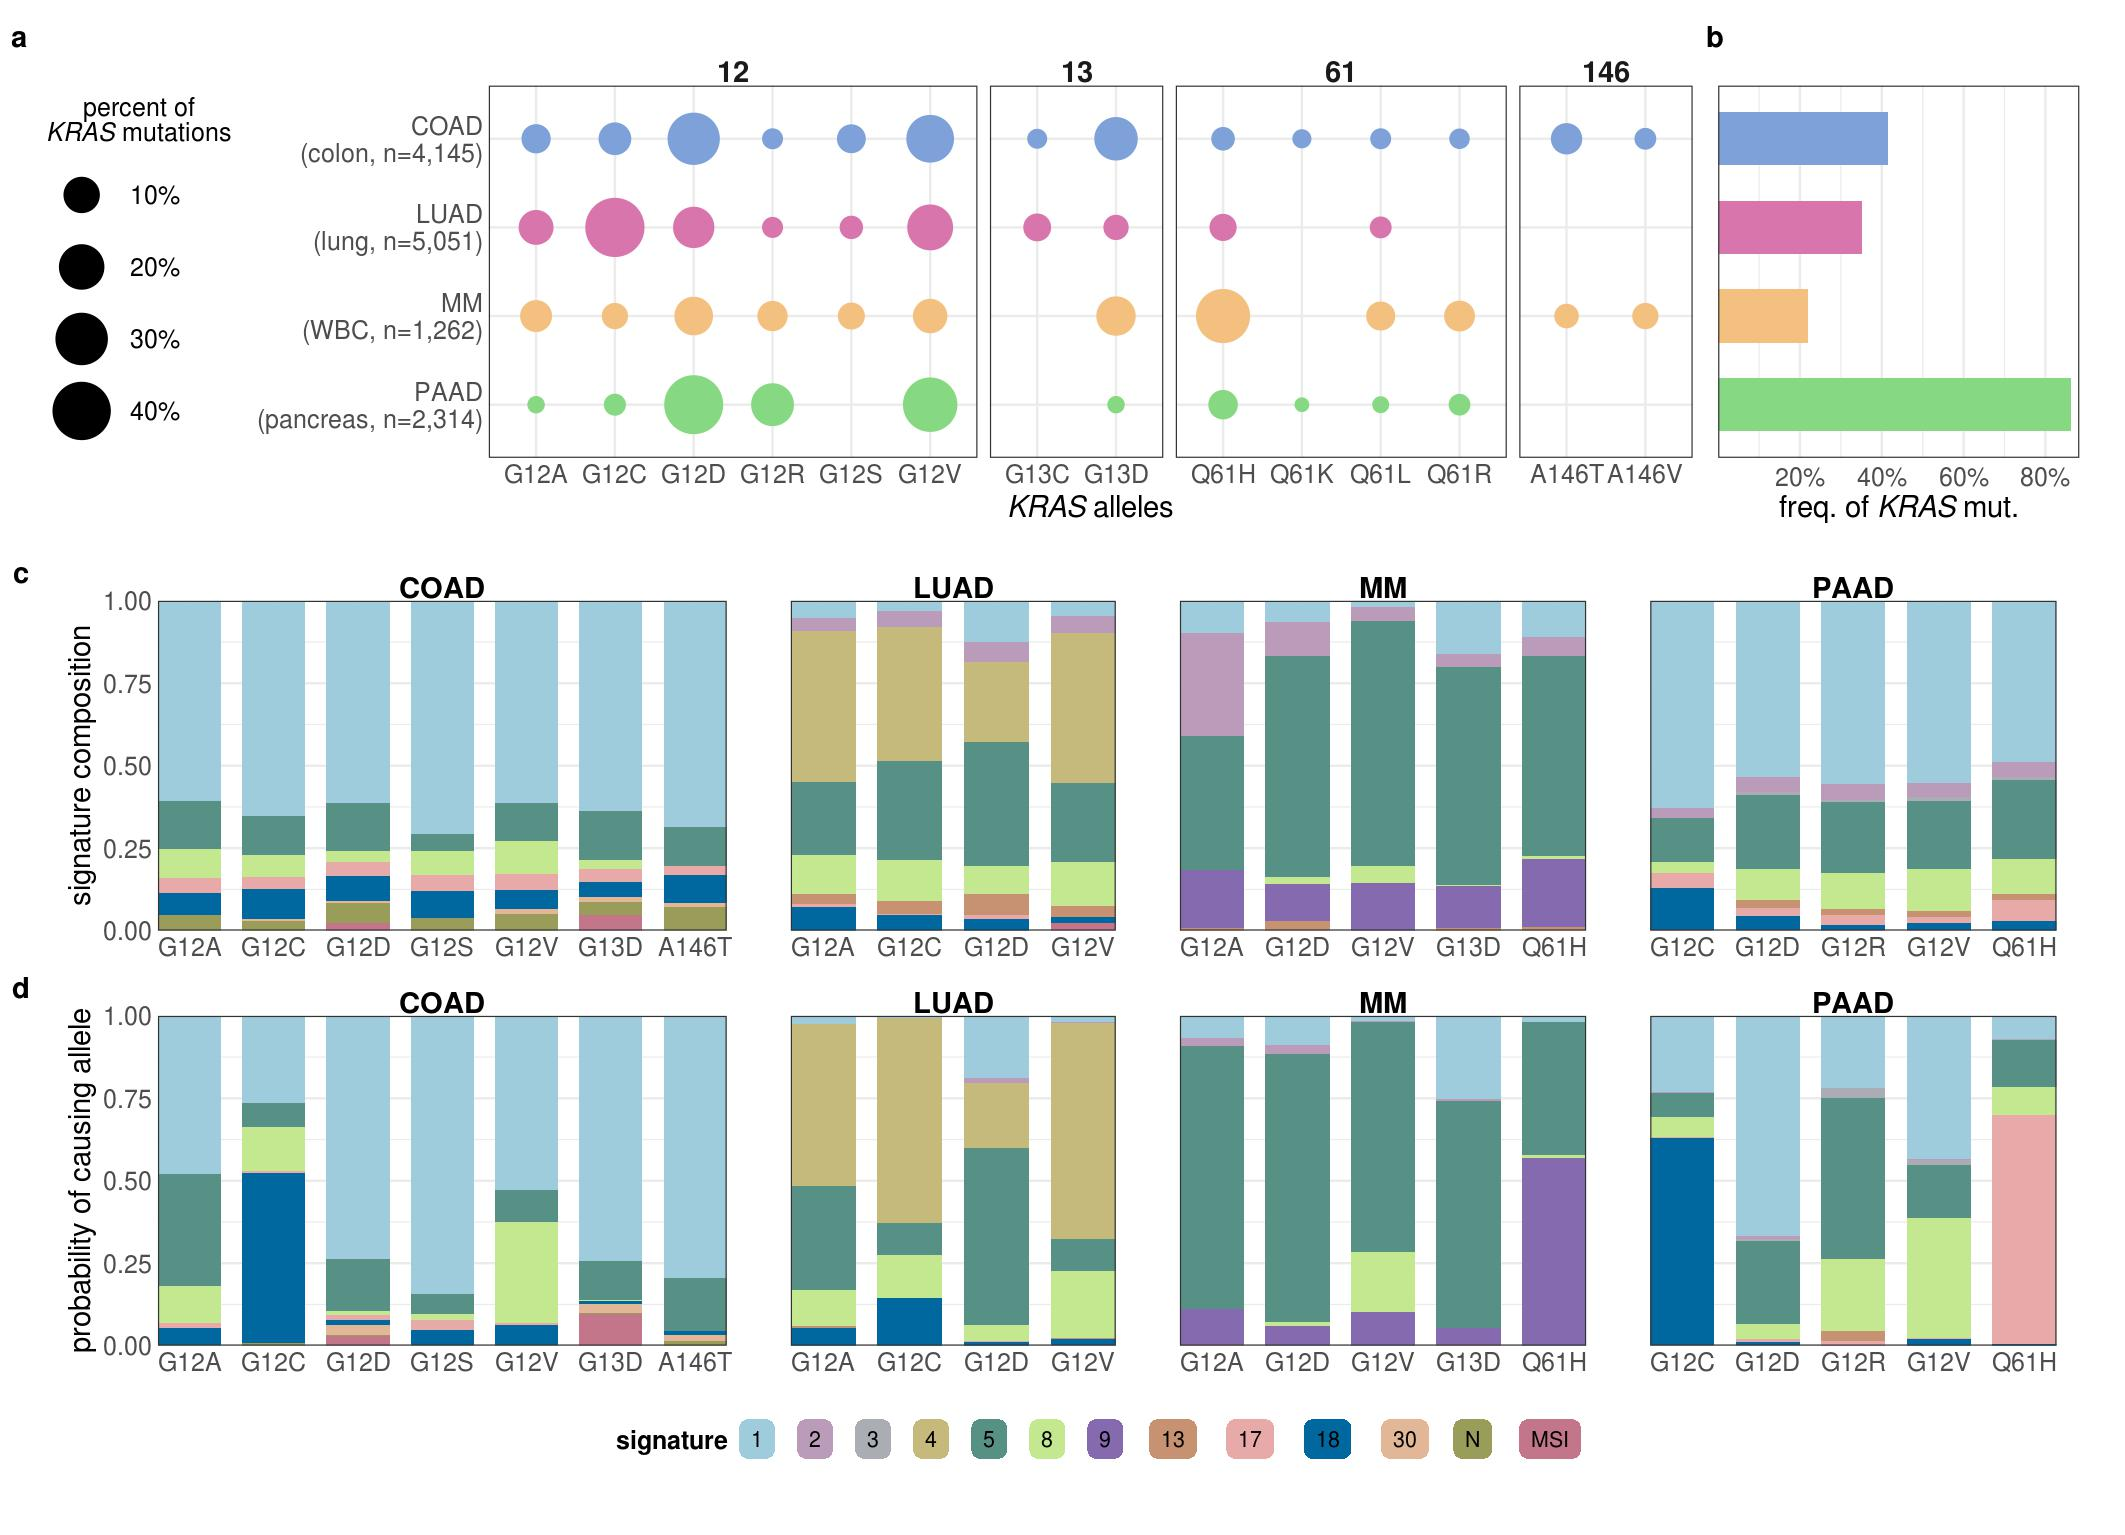
\includegraphics[width=180mm]{figures/Fig_1.jpeg}
\caption{The contribution of mutational processes to \KRAS{} mutagenesis.}
\label{fig:mutational-signatures-main}
\end{figure}
\newpage
\newpage
\noindent Figure 1. \textbf{The contribution of mutational processes to \KRAS{} mutagenesis.}
\textbf{a.} The distribution of \KRAS{} allele frequencies at the four hotspots, codons 12 (left), 13 (middle-left), 61 (middle-right), and 146 (right) in each cancer. The size of the circle reflects the percent of \KRAS{} mutations that are the indicated allele in each cancer. Each cancer is assigned a different color. The number of tumor samples whose sequencing data was collected for this study is indicated along the y-axis. 
\textbf{b.} The frequency of \KRAS{} mutations in each cancer.
\textbf{c.} The average levels of mutational signatures in tumor samples separated by \KRAS{} allele. Each color represents a different mutational signature. Mutational signatures of know etiology are annotated.
\textbf{d.} The average probability of each mutational signature to have caused the \KRAS{} mutation in a tumor sample. This value accounts for the level of each mutational signature in the tumor sample and the ability of the mutational signature to cause the indicated \KRAS{} allele.
\newpage



\begin{figure}[h!]
\centering
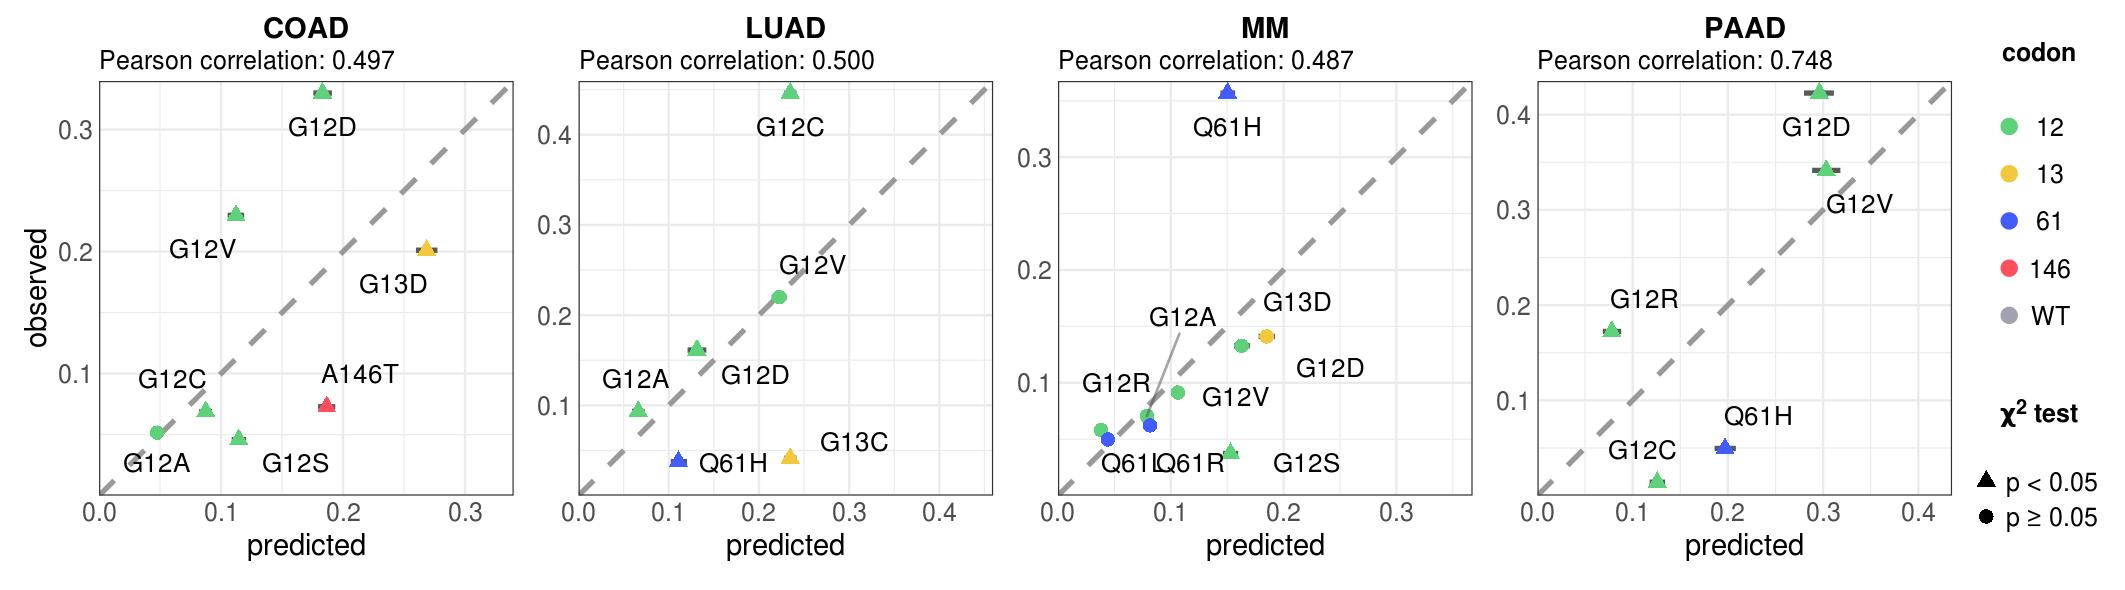
\includegraphics[width=176mm]{figures/Fig_2.jpeg}
\caption{
    \textbf{The predicted frequencies of cancer-specific \KRAS{} alleles.}
    The predicted vs. observed frequency of \KRAS{} alleles for the common alleles of each cancer. $\blacktriangle$ indicates rejection of the null hypothesis that the observed and predicted frequencies are the same (Chi-squared test, p < 0.05). $\bullet$ indicates the failure to reject the null hypothesis (Chi-squared test, p $\ge$ 0.05). Error bars indicate bootstrapped 95\% confidence intervals of the predicted values.
}
\label{fig:obs-vs-pred-main}
\end{figure}
\newpage


\begin{figure}[h!]
\centering
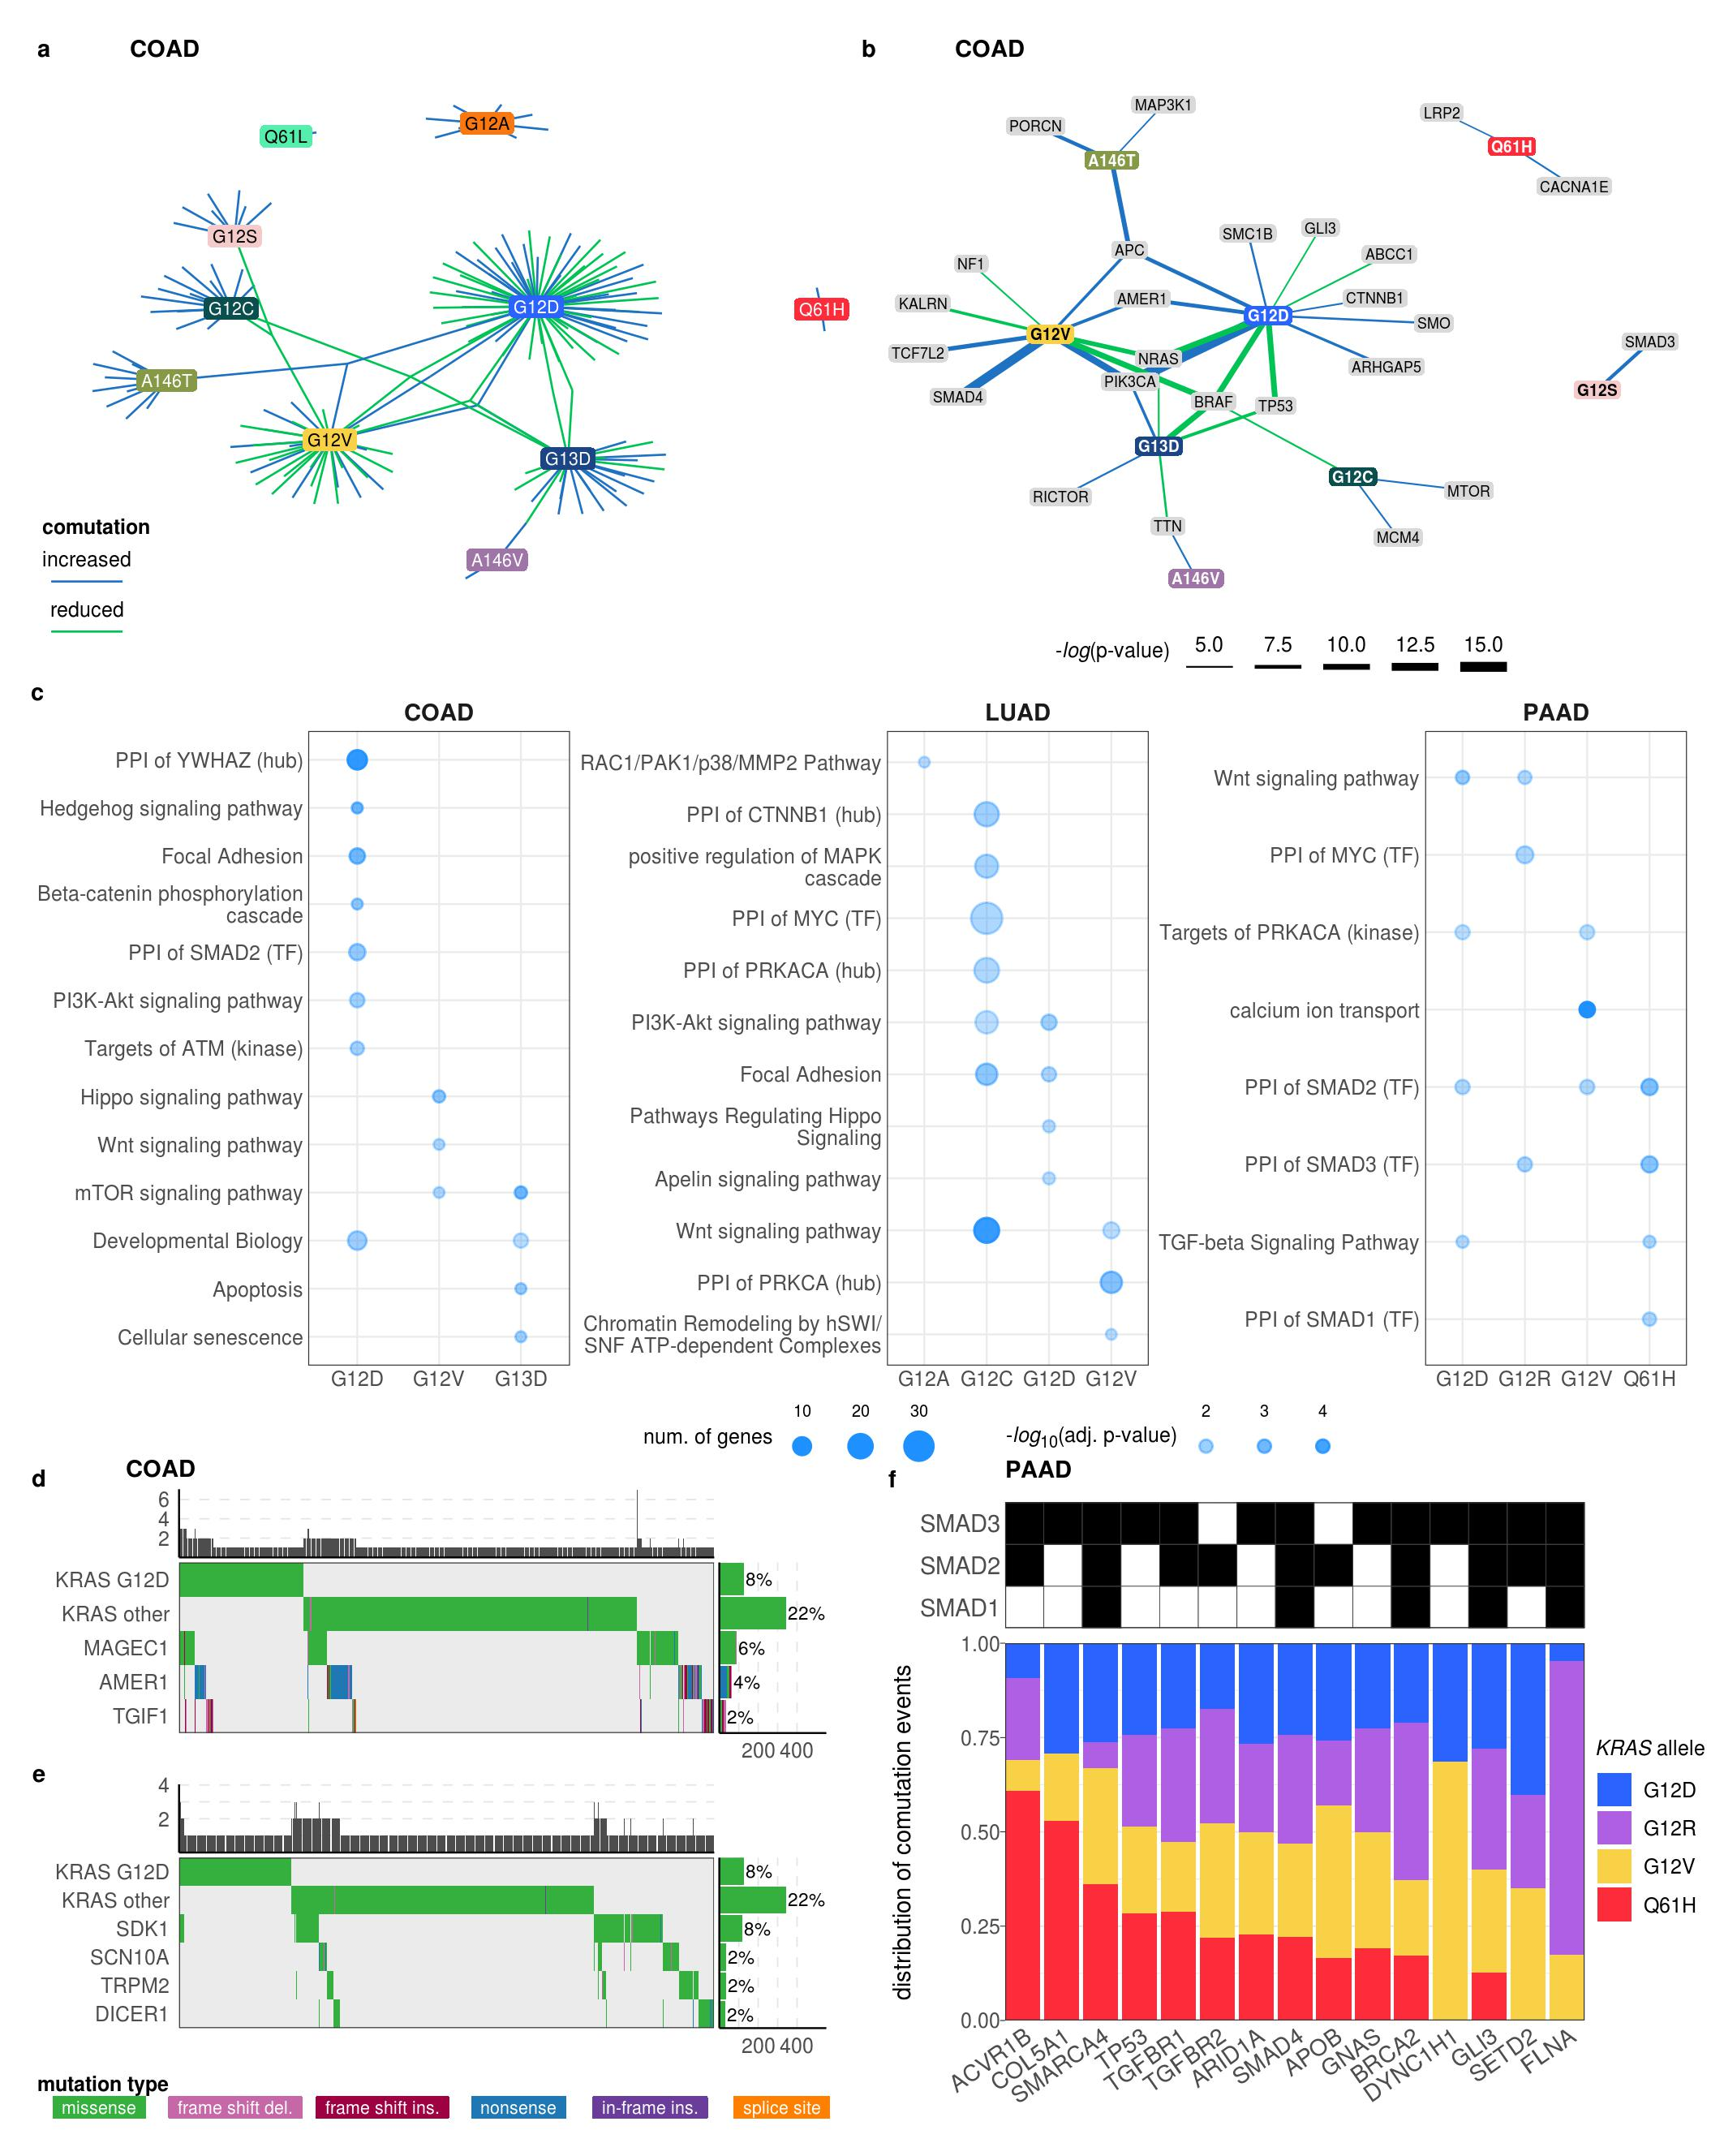
\includegraphics[width=176mm]{figures/Fig_3.jpeg}
\caption{The comutation networks of oncogenic \KRAS{} alleles.}
\label{fig:comutation-main}
\end{figure}
\newpage
\noindent Figure 3. \textbf{The comutation networks of oncogenic \KRAS{} alleles.}
\textbf{a.} The comutation network of the \KRAS{} alleles in COAD with each edge representing a comutation interaction between an allele and another gene. The color of the edge indicates whether the interaction was an increase (blue) or decrease (green) in the frequency of comutation.
\textbf{b.} A subset of the network shown in panel a of genes that encode proteins known to physically interact with \kras{}, are in one of its canonical up- or downstream pathways, or are validated oncogenes. The width of the edge indicates the strength of the association.
\textbf{c.} Cellular functions enriched in the comutation networks of the \KRAS{} alleles in COAD (left), LUAD (center), and PAAD (right). The size of the dot indicates the number of genes in both the function and the comutation network, and the transparency indicates the p-value of the enrichment.
\textbf{d, e.} A visualization of the increased (\textbf{d}) or decreased (\textbf{e}) comutation of select genes with \KRAS{} G12D in COAD. Rows of the central plot represent genes. Each column of the central plot is a different tumor sample. A filled space denotes a mutation of the gene in the sample, the color describing the type of variant. The bar plots above and to the right indicate the marginal values of the central plot.
\textbf{f.} A comparison of the comutation frequencies in PAAD of the genes producing proteins in the PPIN of SMAD1-3. Each column is a gene with a comutation interaction with a \KRAS{} allele and in at least one of the gene sets. The black tiles on top indicate that the gene was in the PPIN of the indicated SMAD protein. The bar plot shows the distribution of the comutation events of each gene across tumor samples with the various \KRAS{} mutations.
\newpage


\begin{figure}[h!]
\centering
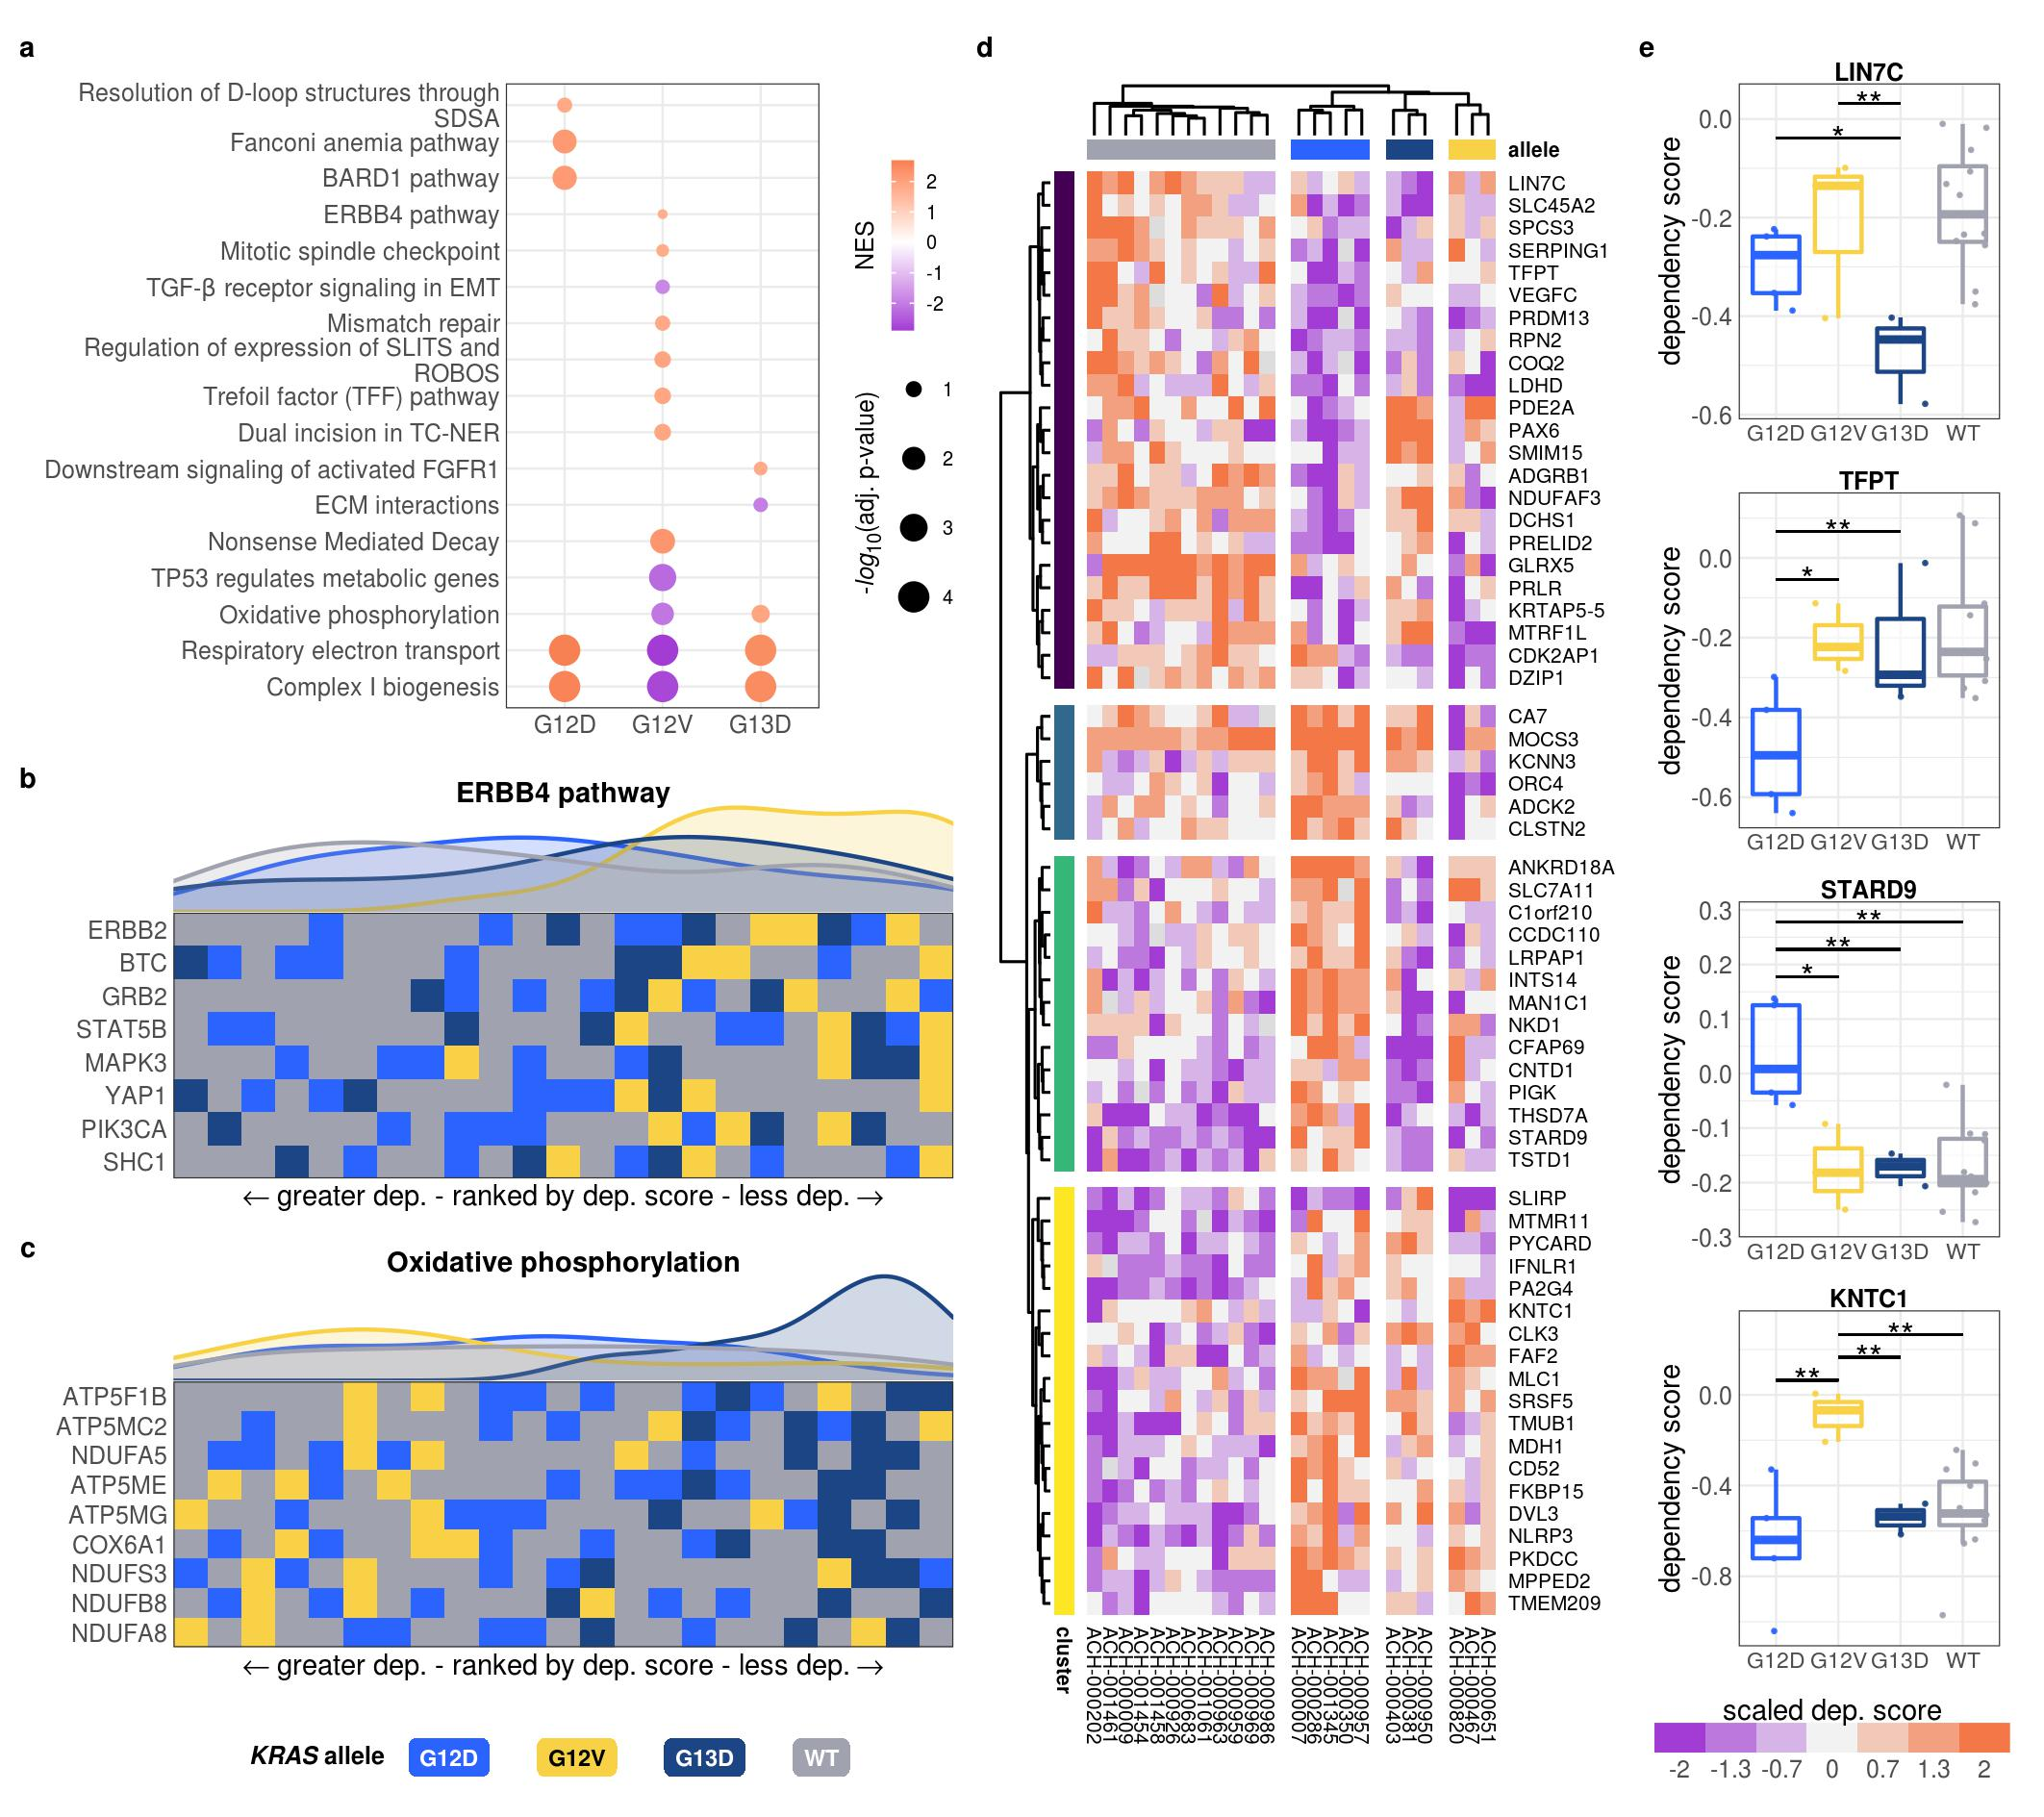
\includegraphics[width=176mm]{figures/Fig_4.jpeg}
\caption{Allele-specific genetic dependencies in COAD cell lines.}
\label{fig:coad-dependency-main}
\end{figure}
\newpage
\newpage
\noindent Figure 4. \textbf{Allele-specific genetic dependencies in COAD cell lines.}
\textbf{a.} Gene sets with significant enrichment for increased (lower dependency score; purple) or reduced (higher dependency score; orange) genetic dependency in COAD cell lines. The size of the dot relates the p-value of the association and the color indicated the strength of the enrichment ("normalized enrichment score").
\textbf{b, c.} Heatmaps ranking the cell lines by dependency score of the genes at the leading edge of enrichment for two gene sets. Each row represents a gene and each cell represents a cell line colored by its \KRAS{} allele. The cell lines are arranged in ranking order by their dependency score for the gene. Thus, each column indicates a rank. The line plots above the heatmaps indicate the representation (density) of each \KRAS{} allele at each rank across the genes.
\textbf{d.} Hierarchically clustered heatmaps of the genes that demonstrated differential genetic dependency amongst cell lines of different \KRAS{} alleles. Each column is a cell line labeled by its DepMap identifier and each row is a gene.
\textbf{e.} Examples of genes that demonstrated differential genetic dependency amongst cell lines of different \KRAS{} alleles (pairwise t-tests; *: p<0.05, **: p<0.01, ***: p<0.001; p-values were adjusted using the Benjamini-Hochberg FDR correction method).
\newpage


\begin{figure}[h!]
\centering
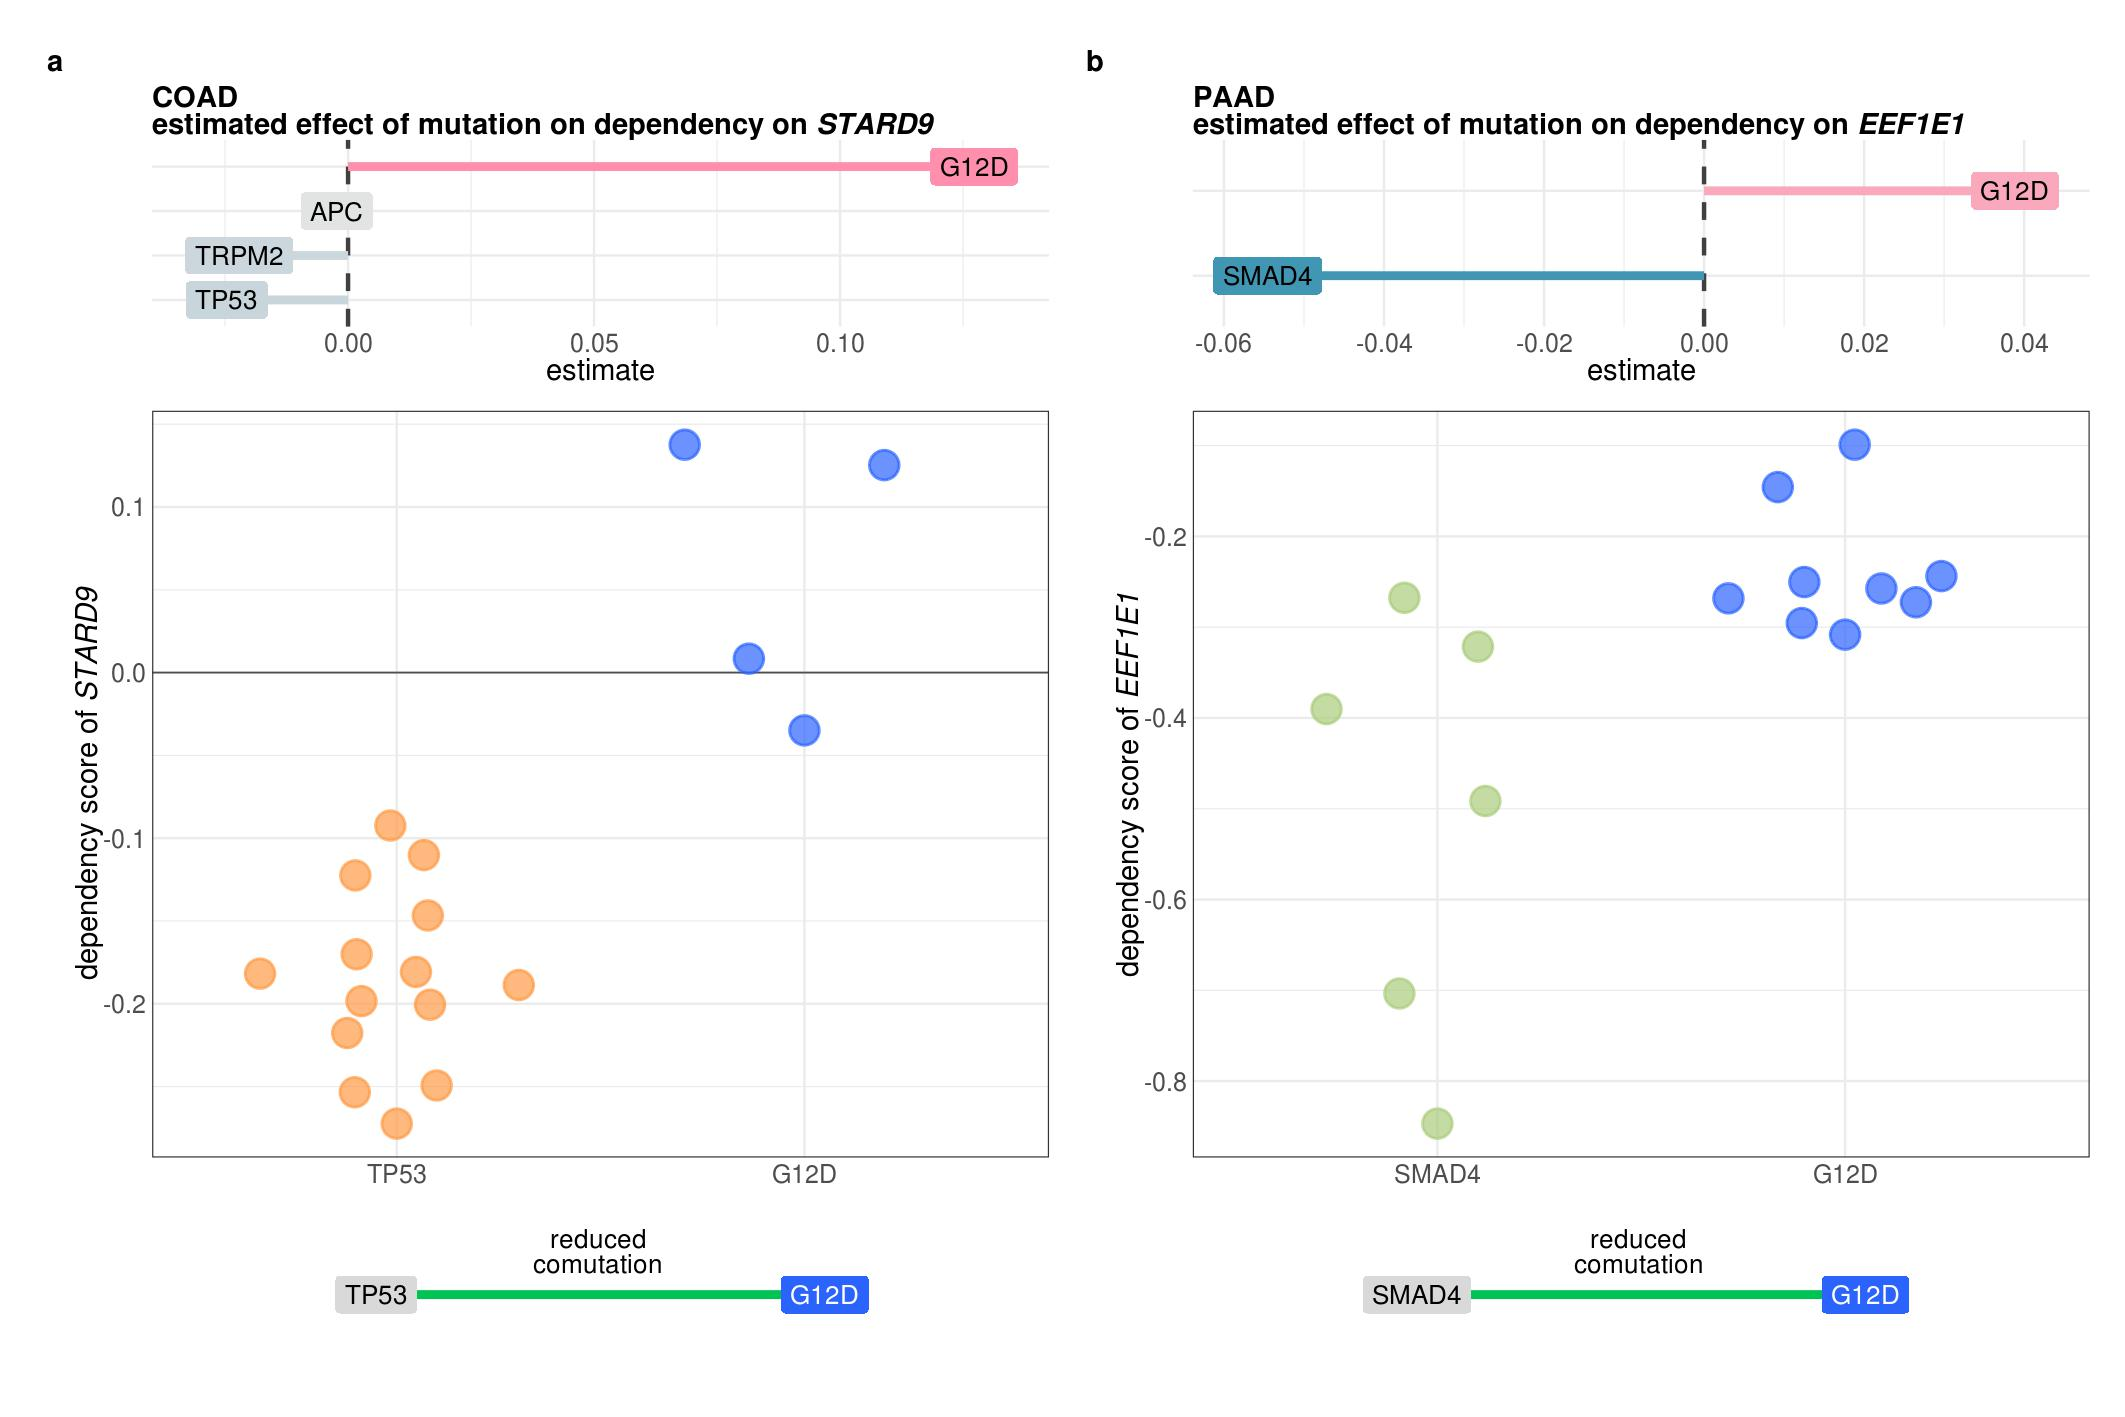
\includegraphics[width=180mm]{figures/Fig_5.jpeg}
\caption{Integration of comutation and genetic dependency results.}
\label{fig:results-integration-main}
\end{figure}
\newpage
\noindent Figure 5. \textbf{Integration of comutation and genetic dependency results.}
\textbf{a.} (In progress. The above image is just a temporary placeholder.)
\newpage



%-------------- SUPPLEMENTAL FIGURES ----------------%

\beginsupplement
\makeatletter
\renewcommand{\fnum@figure}{Supplementary \figurename~\thefigure}
\makeatother



\begin{figure}[h!]
\centering
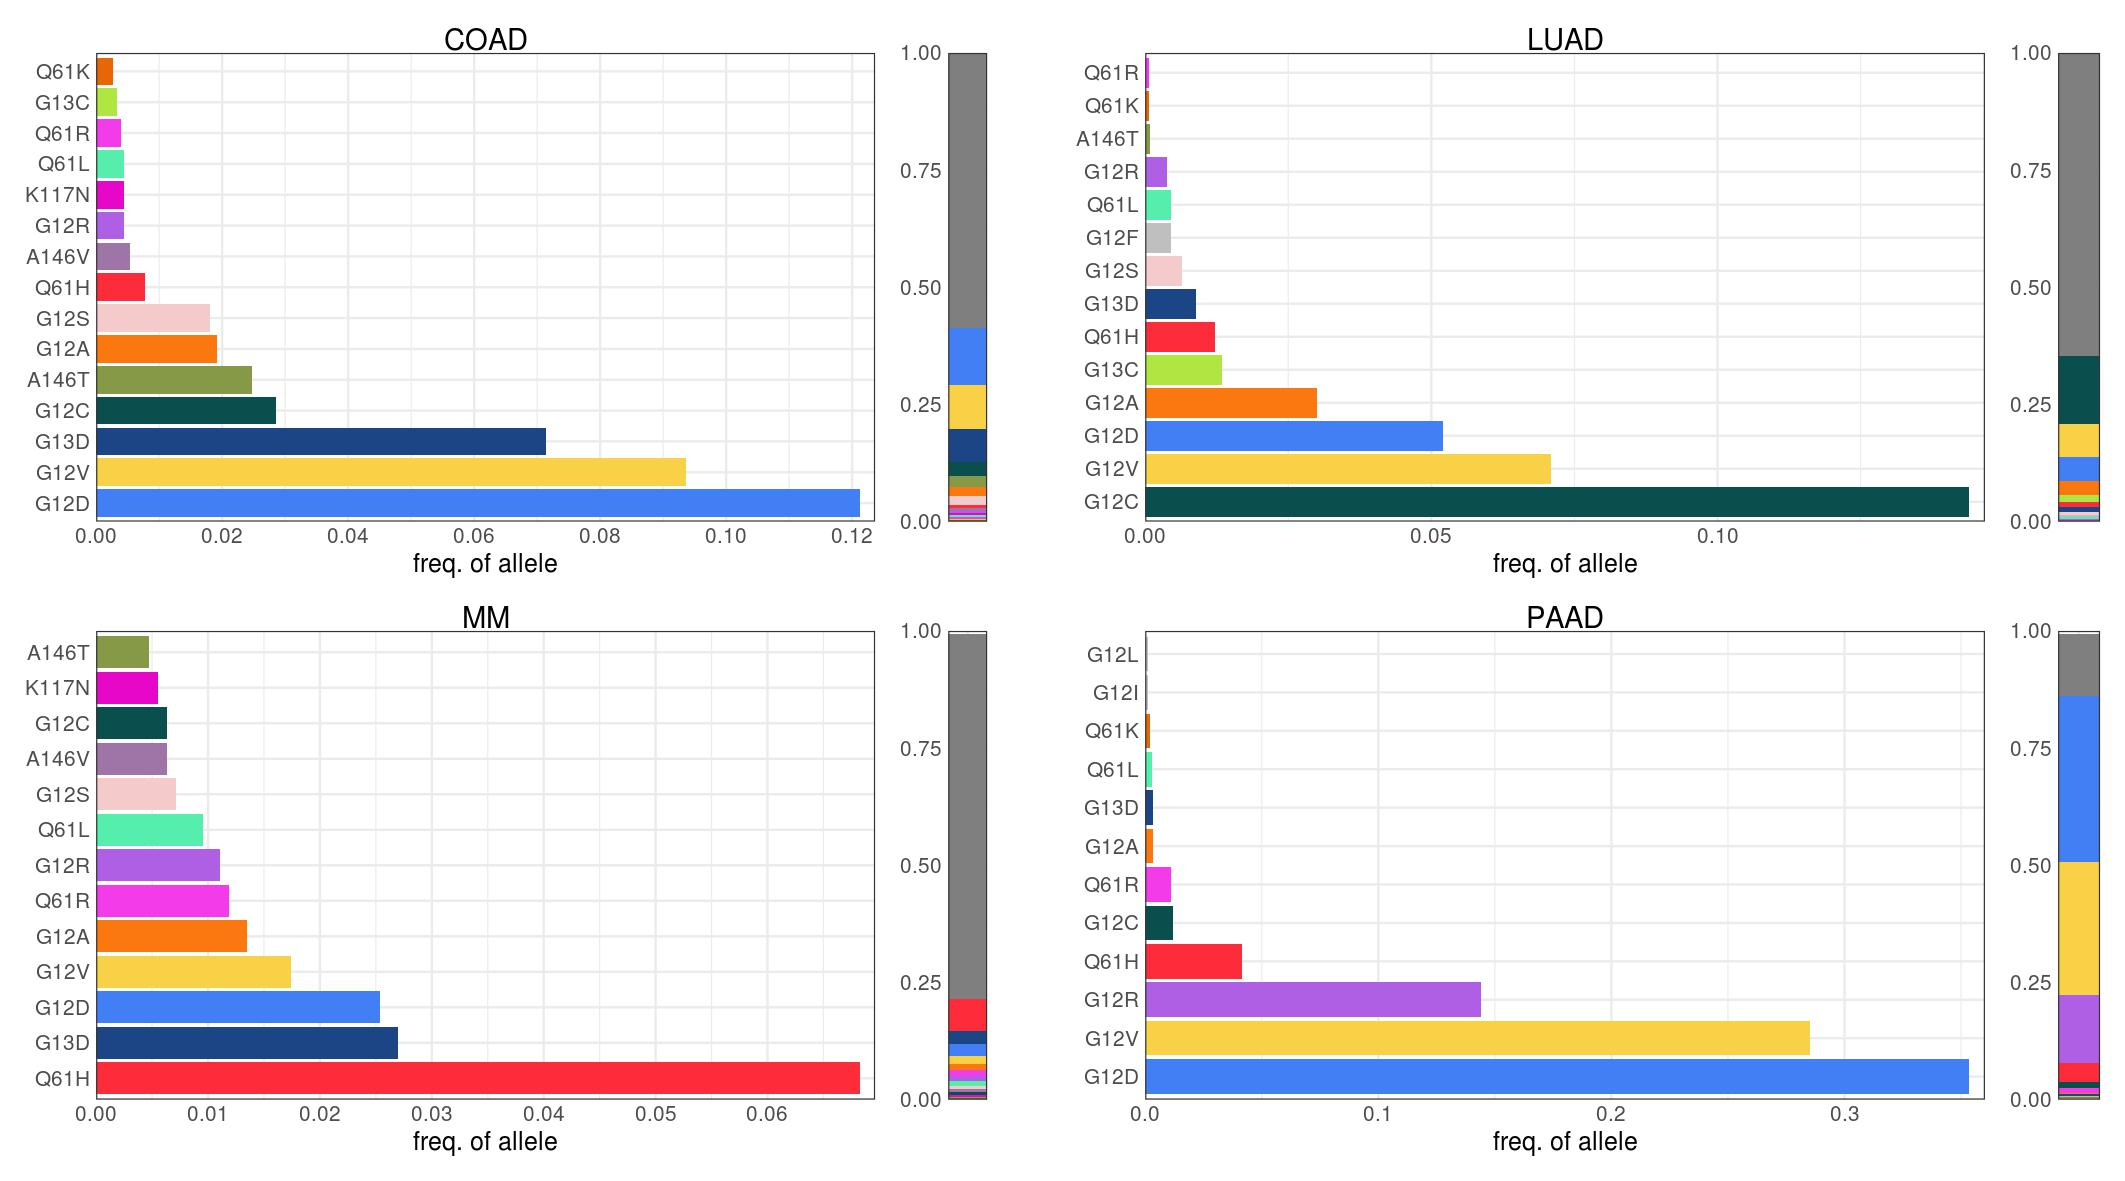
\includegraphics[width=180mm]{figures/Supp_Fig_1.jpeg}
\caption{
    \textbf{Mutational signatures in tumor samples.}
    \textbf{a, b.} The detected level of the mutational signatures in each tumor sample. In \textbf{a}, each tumor sample is a column.
    \textbf{c.} The average levels of clock (signatures 1 and 5) and non-clock (all other signatures) in the tumor samples.
}
\label{sfig:mutational-signatures-supp}
\end{figure}
\newpage


\begin{figure}[h!]
\centering
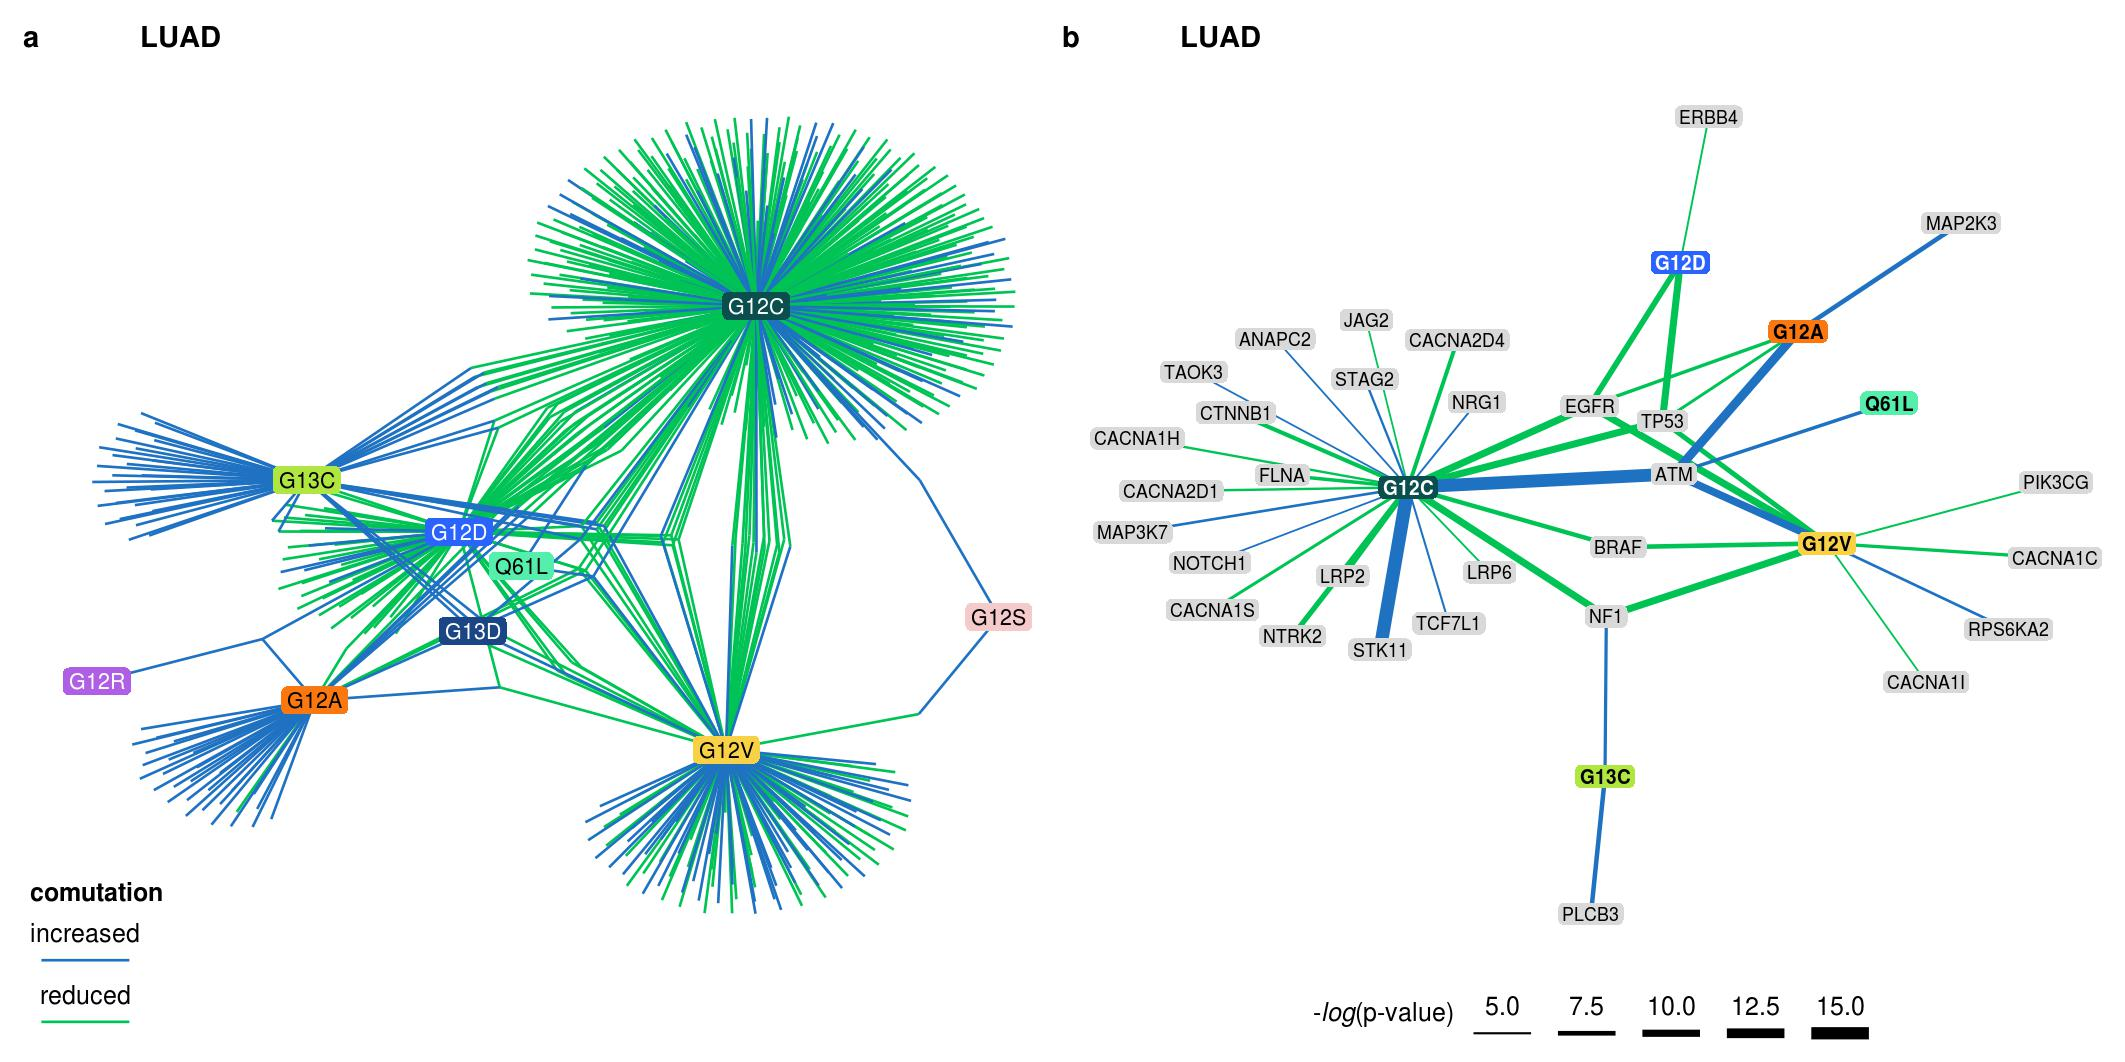
\includegraphics[width=180mm]{figures/Supp_Fig_2.jpeg}
\caption{
    \textbf{The predicted frequencies of all oncogenic \KRAS{} alleles in each cancer.}
    The predicted vs. observed frequency of \KRAS{} alleles in each cancer for all \KRAS{} alleles demonstrated to drive any of the four cancers. The \KRAS{} alleles included in the calculation were found mutated frequently in at least one of the four cancer types. $\blacktriangle$ indicates rejection of the null hypothesis that the observed and predicted frequencies are the same (Chi-squared test, p < 0.05). $\bullet$ indicates the failure to reject the null hypothesis (Chi-squared test, p $\ge$ 0.05). Error bars indicate bootstrapped 95\% confidence intervals of the predicted values.
}
\label{sfig:obs-vs-pred-supp}
\end{figure}
\newpage


\begin{figure}[h!]
\centering
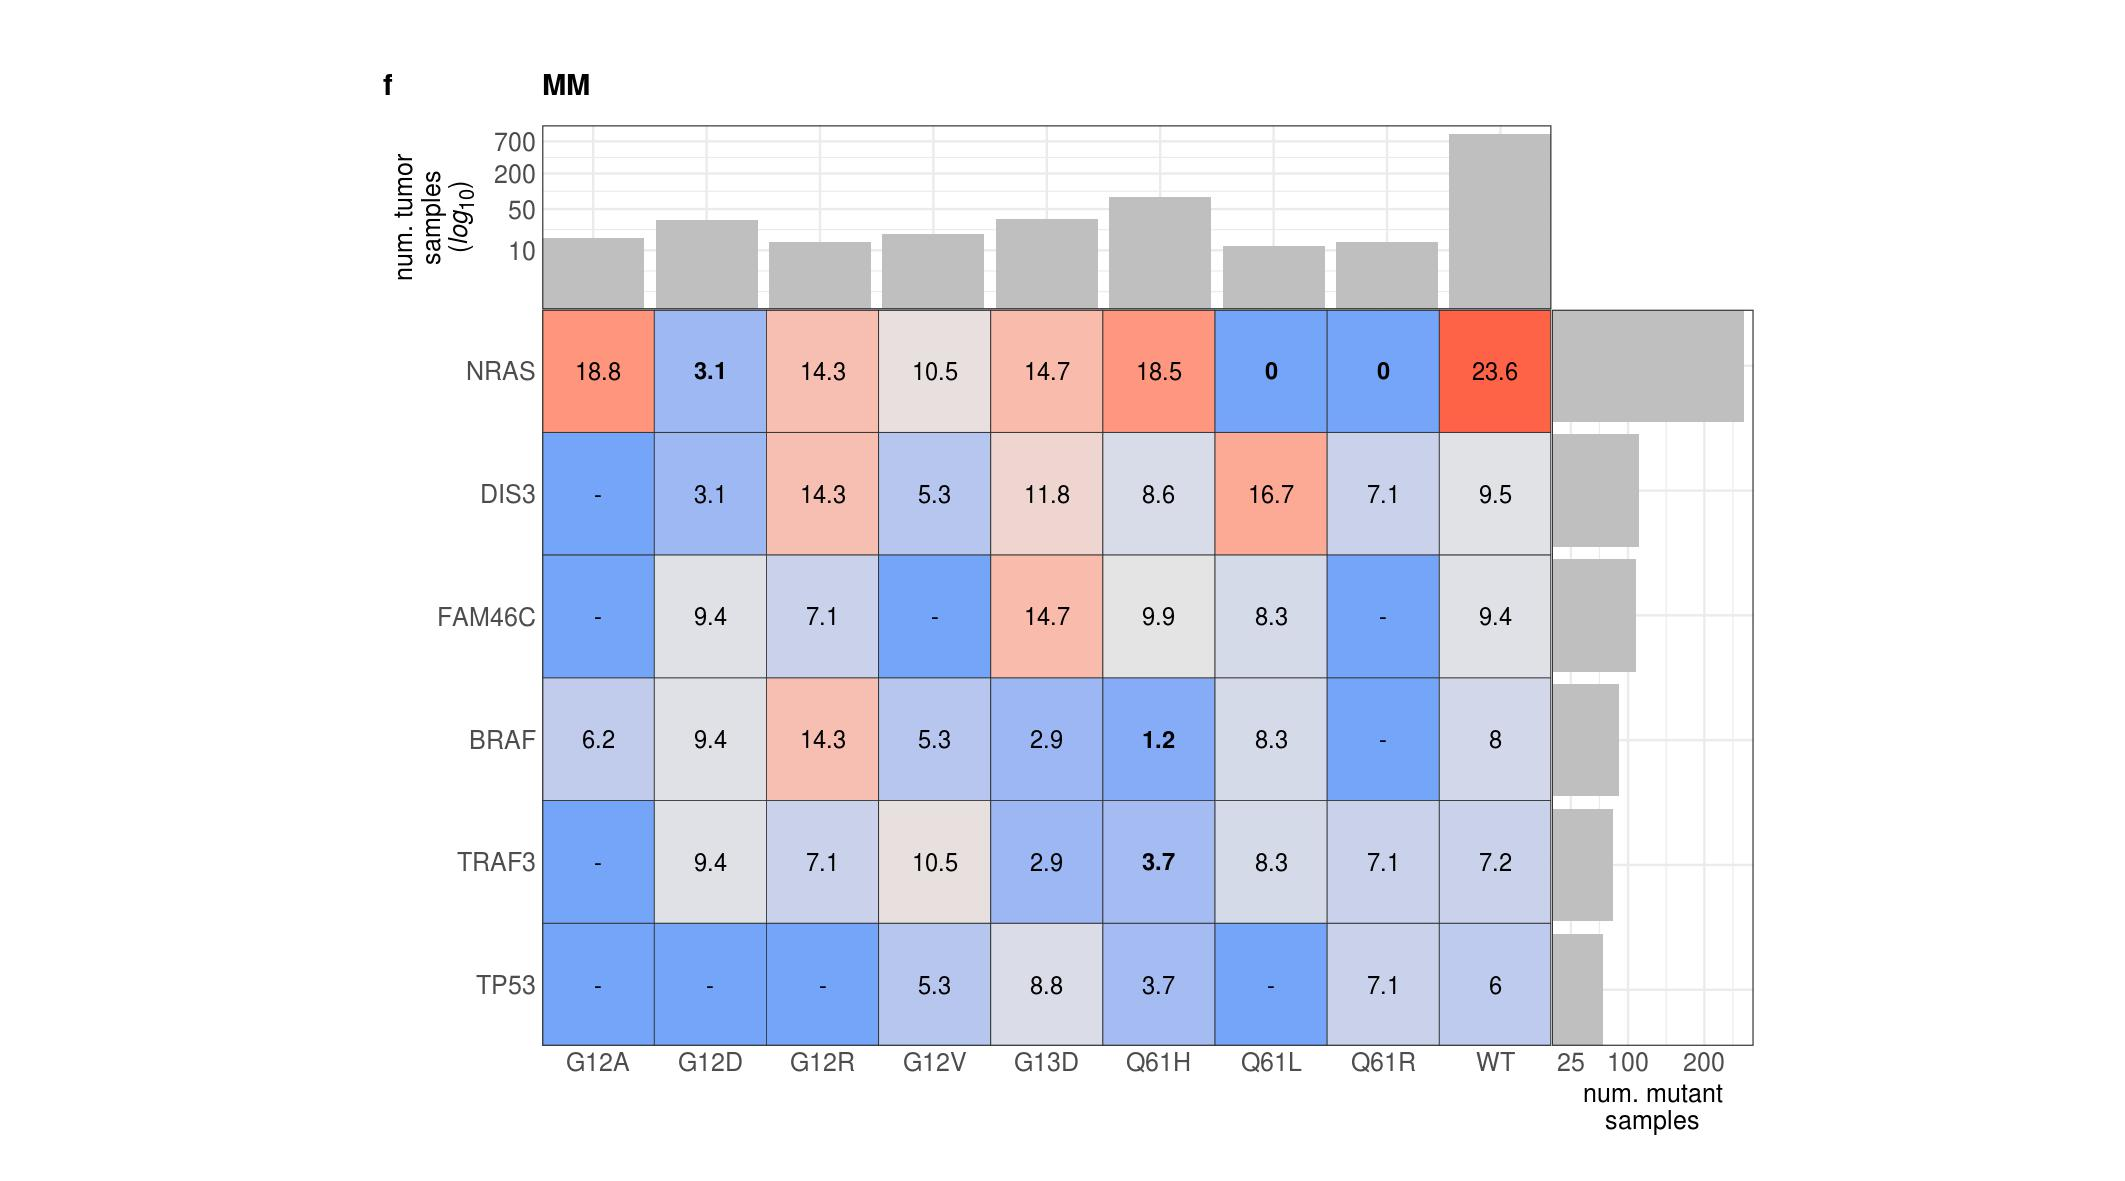
\includegraphics[width=180mm]{figures/Supp_Fig_3.jpeg}
\caption{
    \textbf{The comutation networks of \KRAS{} alleles in LUAD.}
    \textbf{a.} The comutation network of the \KRAS{} alleles in LUAD where each edge represents a comutation interaction between an allele and another gene. The color of the edge indicates whether the interaction was an increase (blue) or decrease (green) in the frequency of comutation.
    \textbf{b.} A subset of the network shown in \textbf{a} of genes in one of its canonical up- or downstream signaling pathways. The width of the edge indicates the strength of the association.
}
\label{sfig:luad-comutation-network}
\end{figure}
\newpage


\begin{figure}[h!]
\centering
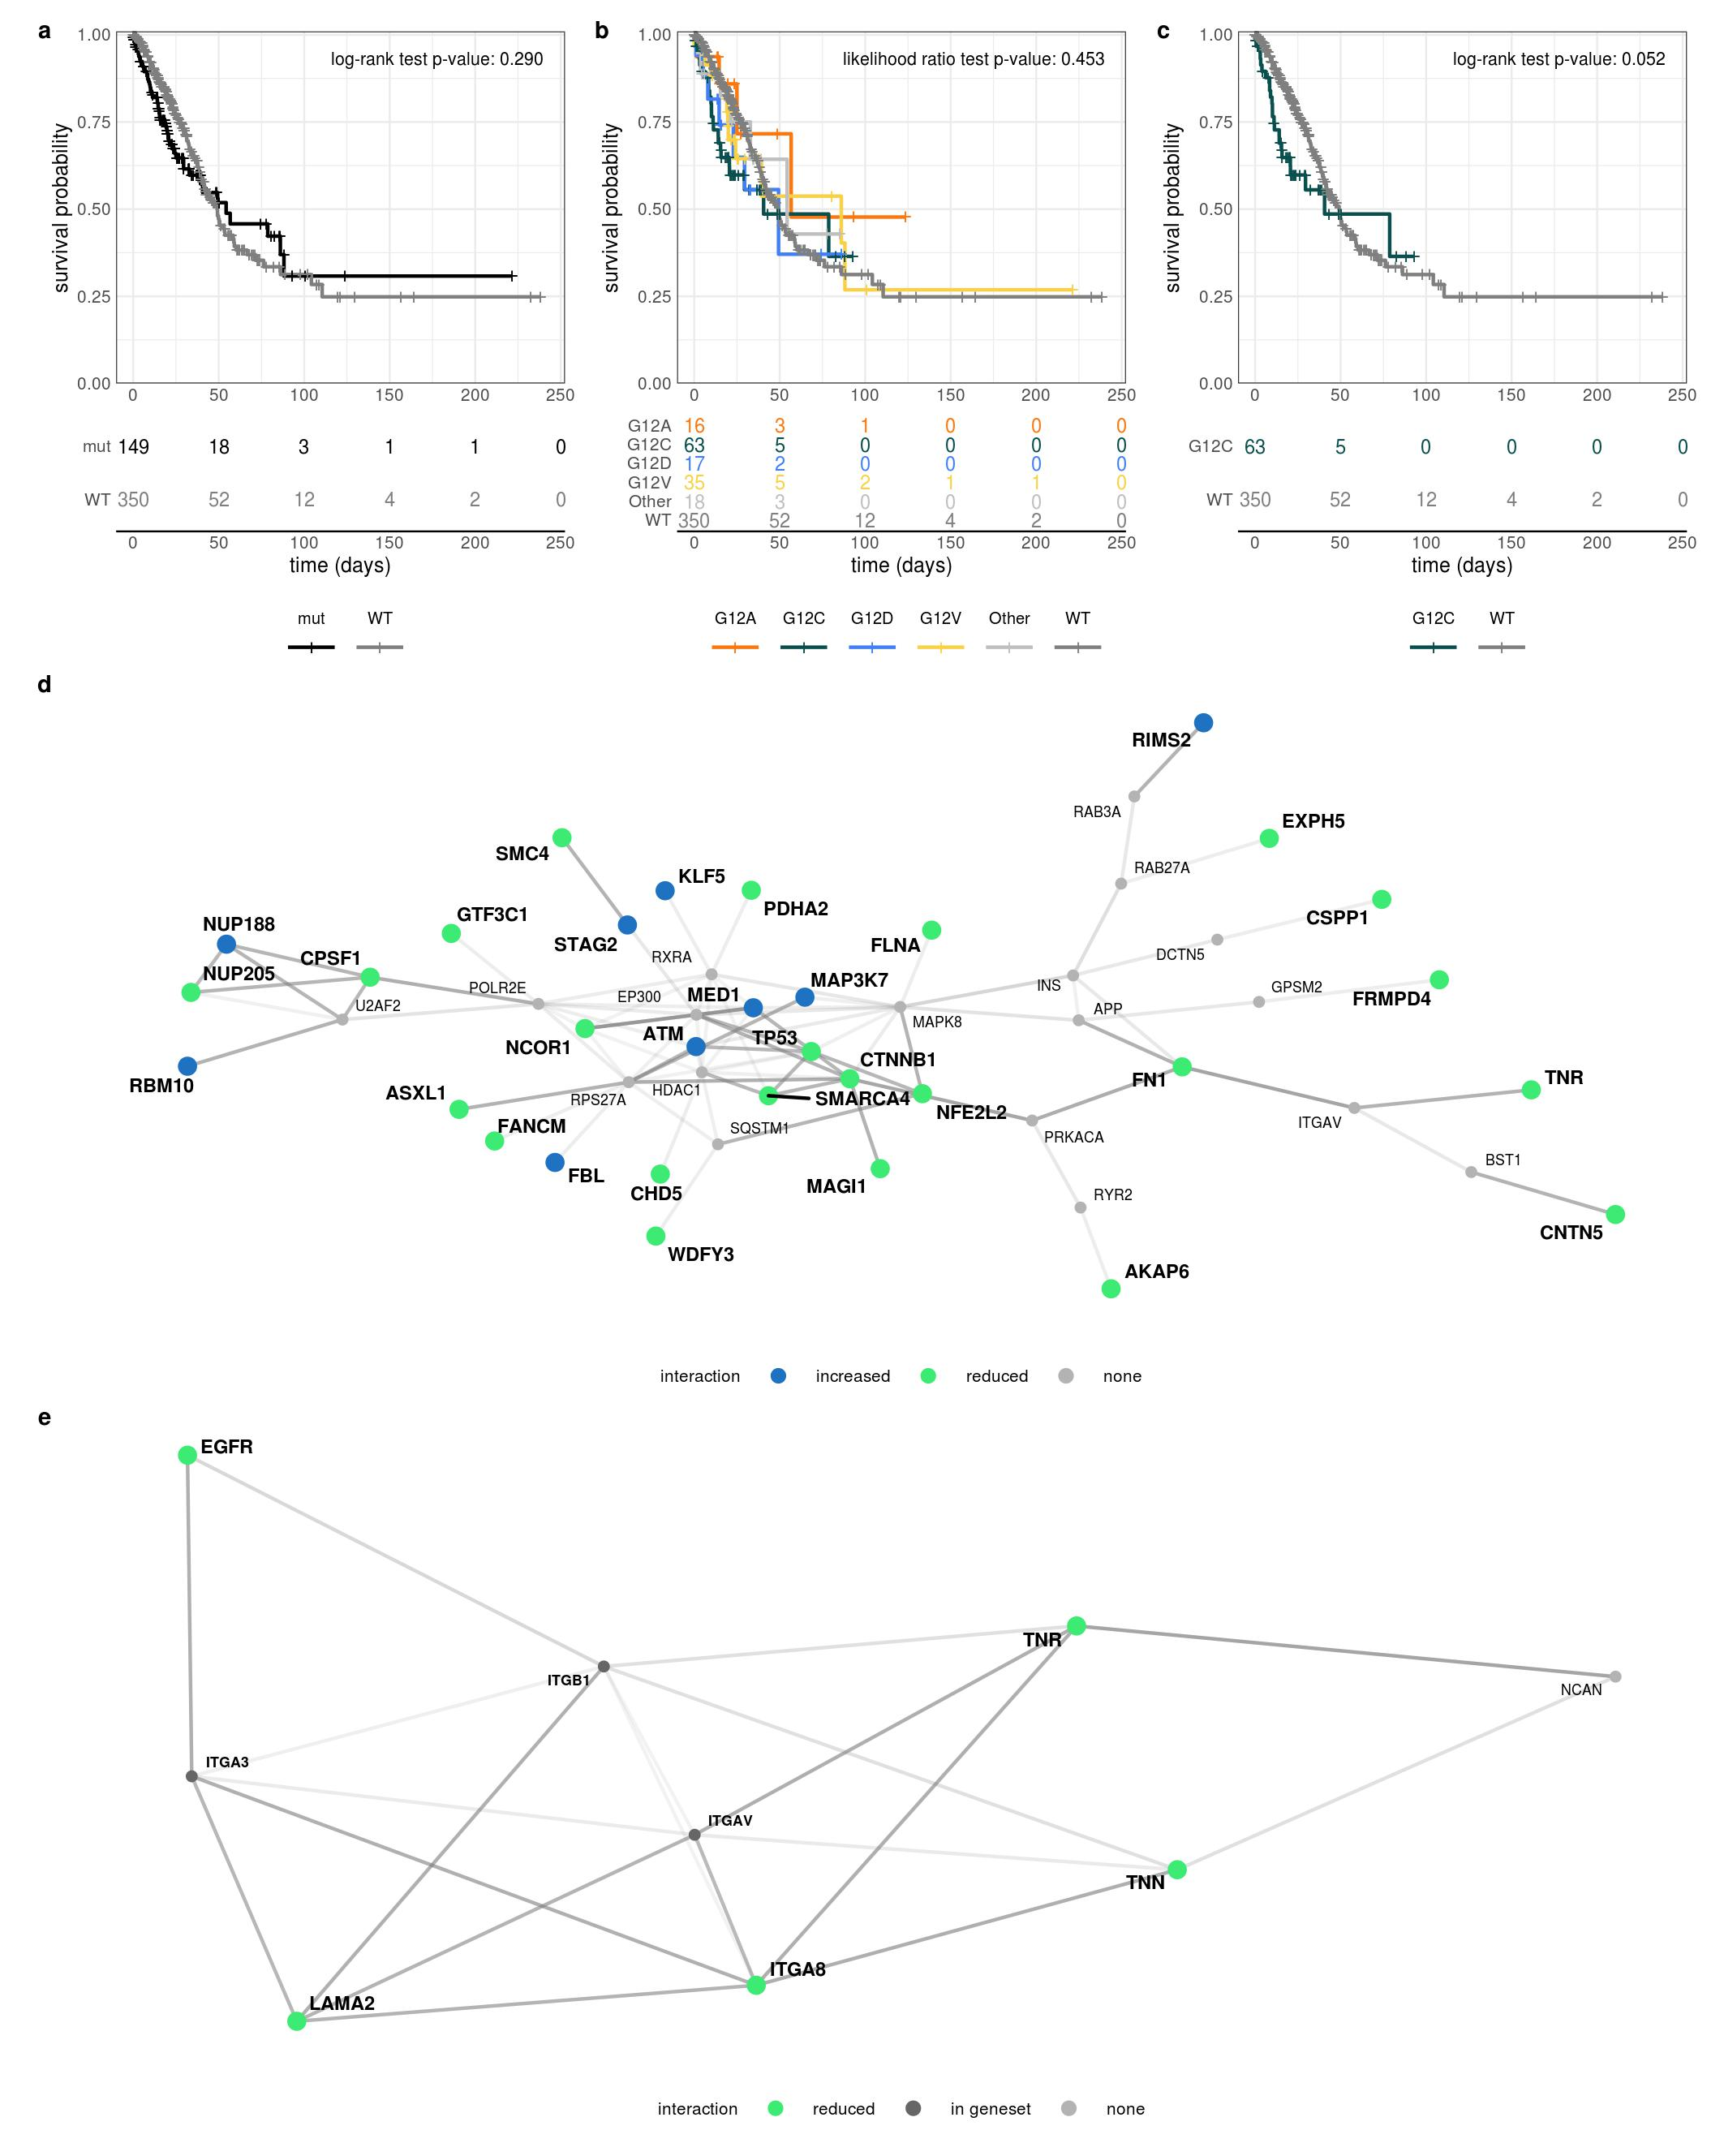
\includegraphics[width=180mm]{figures/Supp_Fig_4.jpeg}
\caption{
    \textbf{The comutation frequencies between known MM driver genes and \KRAS{} alleles.} The color is correlated with the comutation frequency (the fraction of cells with the \KRAS{} allele that also have a mutation in the other driver gene), indicated in each cell. Bold percent values indicate statistical significance of a comutation interaction (see Methods). The bar plot along the top indicates the number of samples with the \KRAS{} allele, and the bar plot on the right indicates the number of samples with a mutation in the gene.
}
\label{sfig:mm-comutation-heatmap}
\end{figure}
\newpage


\begin{figure}[h!]
\centering
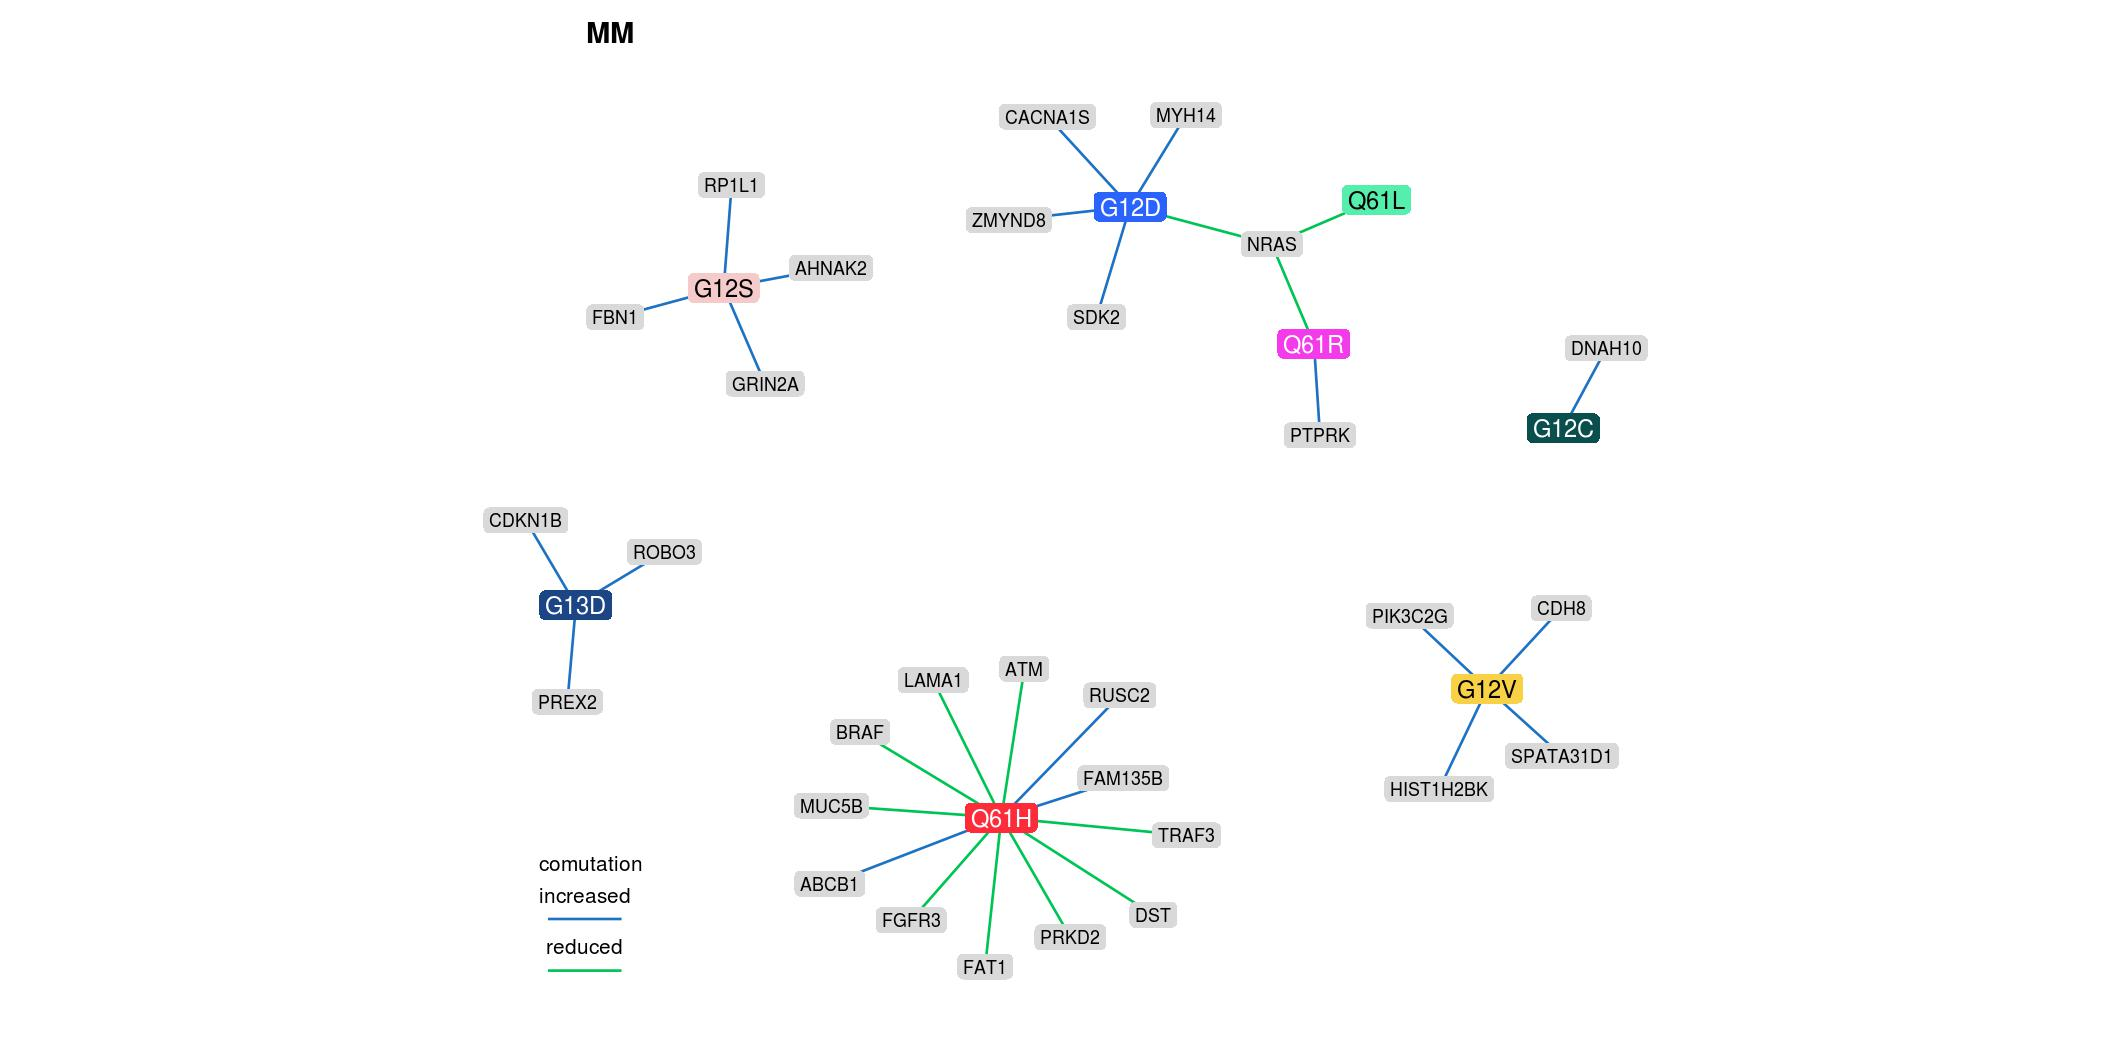
\includegraphics[width=180mm]{figures/Supp_Fig_5.jpeg}
\caption{
    \textbf{The comutation networks of \KRAS{} alleles in PAAD.}
    \textbf{a.} The comutation network of the \KRAS{} alleles in PAAD where each edge represents a comutation interaction between an allele and another gene. The color of the edge indicates whether the interaction was an increase (blue) or decrease (green) in the frequency of comutation.
    \textbf{b.} A subset of the network shown in \textbf{a} of genes known to physically interact with \KRAS{}, are in one of its canonical up- or downstream pathways, or are validated oncogenes. The width of the edge indicates the strength of the association.
    \textbf{c.} The log-odds of comutation between \KRAS{} alleles and other genes that had detectable opposing comutation interactions with multiple alleles.
}
\label{sfig:paad-comutation-network}
\end{figure}
\newpage


\begin{figure}[h!]
\centering
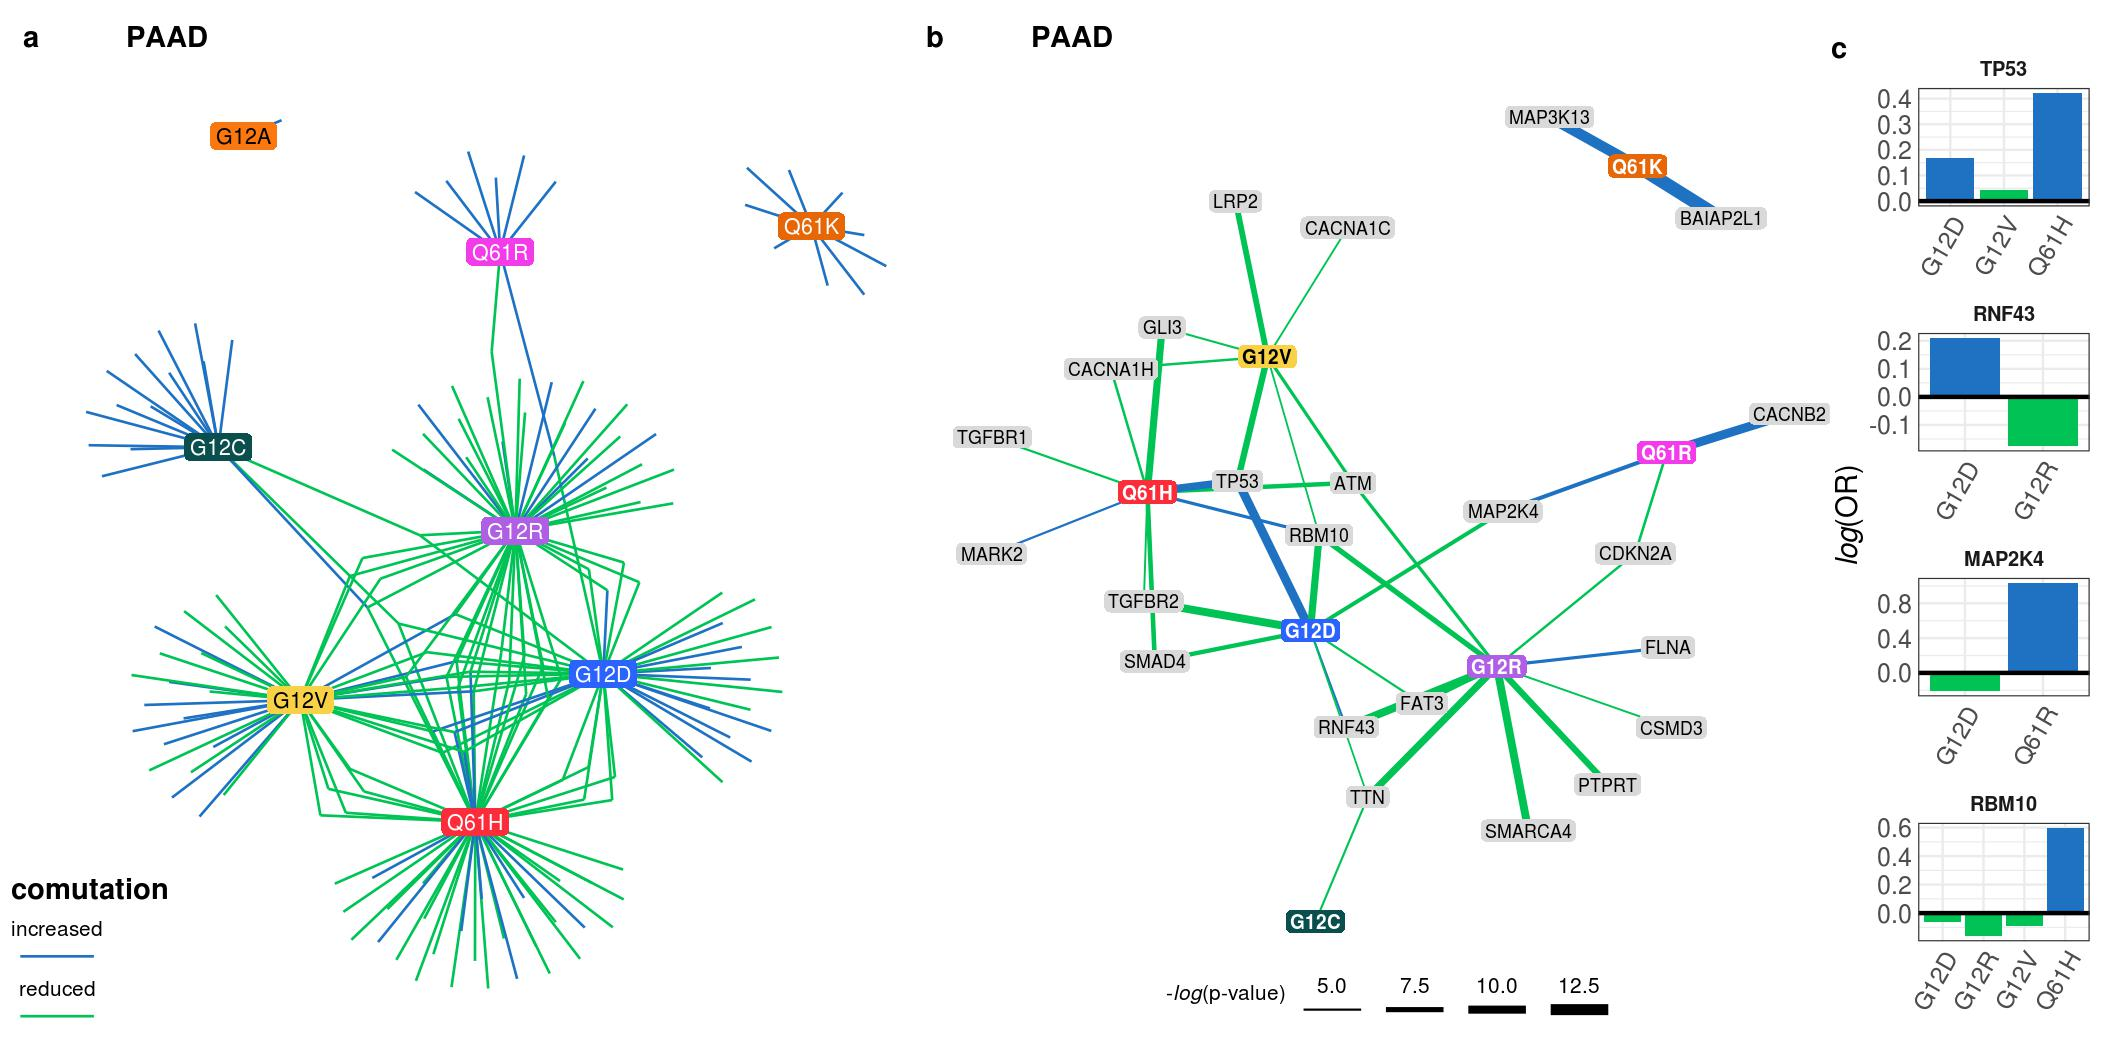
\includegraphics[width=85mm]{figures/Supp_Fig_6.jpeg}
\caption{Allele-specific genetic dependencies on cellular processes and pathways in PAAD cell lines.}
\label{sfig:paad-dependency-gsea}
\end{figure}
\newpage
\noindent Supplementary Figure 6. \textbf{Cellular processes enriched for greater or lesser genetic dependencies in PAAD cell lines separated by \KRAS{} allele.}
\textbf{a.} Gene sets with significant enrichment for increased (lower dependency score; purple) or reduced (higher dependency score; orange) genetic dependency in PAAD cell lines. The size of the dot relates the p-value of the association, and the color indicates the strength of the enrichment.
\textbf{b, c, d.} Heatmaps ranking the cell lines by dependency score of genes at the leading edge of enrichment for three gene sets in PAAD. Each row represents a gene and each cell represents a cell line colored by its \KRAS{} allele. The cell lines were arranged in ranking order by their dependency score for the gene. Thus, each column indicates a rank. The line plots above the heatmaps indicate the representation (density) of each \KRAS{} allele at each rank across the genes.
\newpage


\begin{figure}[h!]
\centering
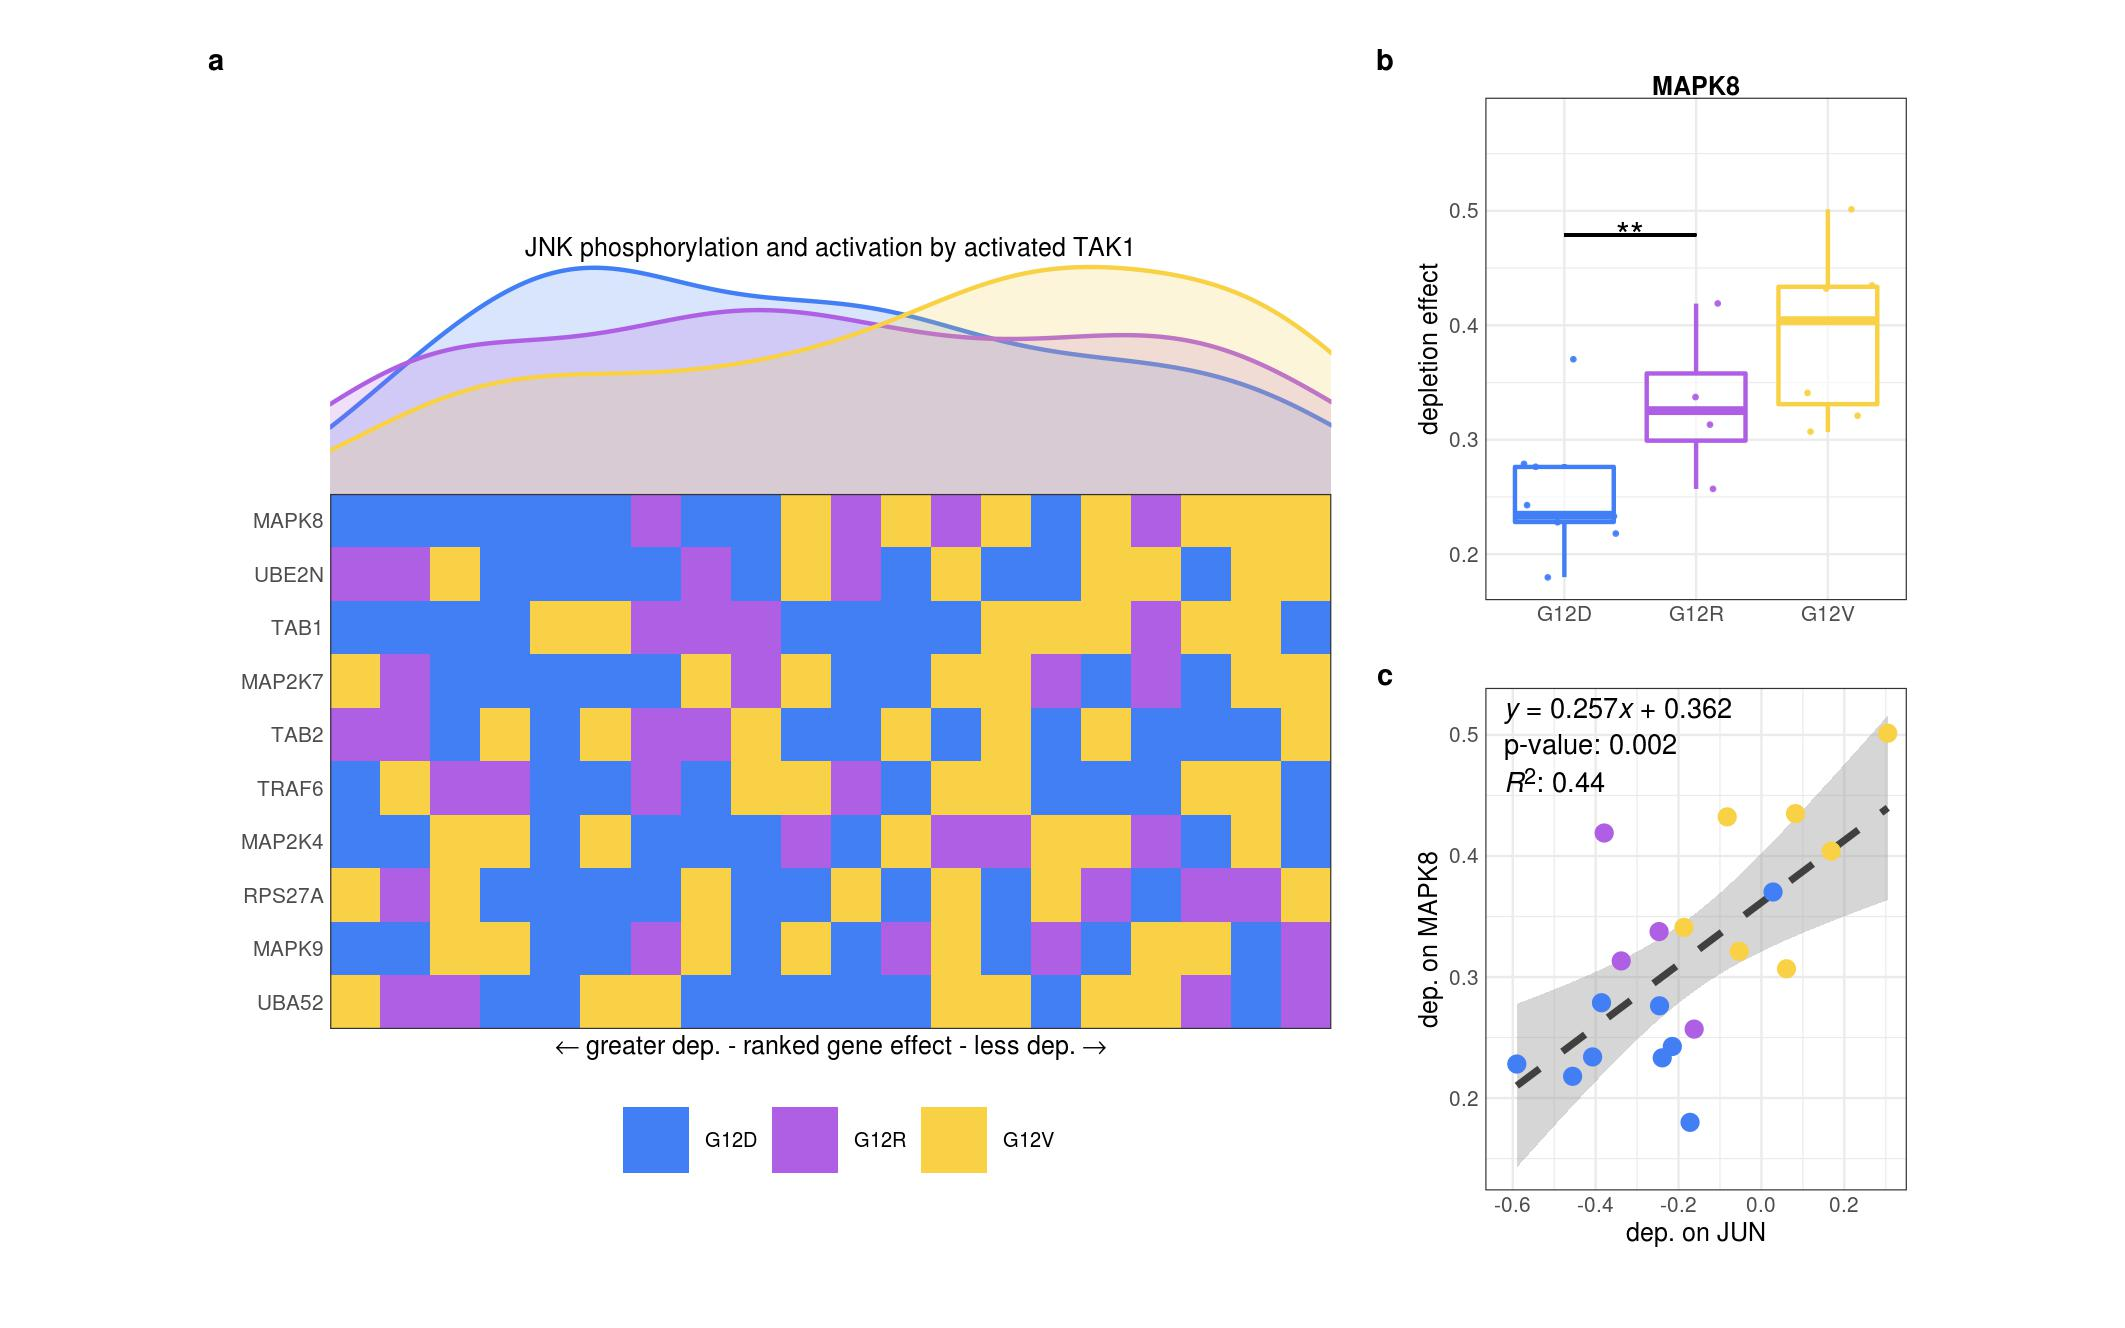
\includegraphics[width=88mm]{figures/Supp_Fig_7.jpeg}
\caption{
    \textbf{Individual genes with differential genetic dependency by \KRAS{} allele in PAAD cell lines.}
    \textbf{a.} Clustered heatmaps of the genes that demonstrated differential genetic dependency amongst cell lines of different \KRAS{} alleles in PAAD cell lines. Each column is a cell line labeled by its DepMap ID and each row is a gene.
    \textbf{b.} Examples of genes that demonstrated differential genetic dependency amongst cell lines of different \KRAS{} alleles in PAAD (pairwise t-tests; *: p < 0.05, **: p < 0.01, ***: p < 0.001; p-values were adjusted using the Benjamini-Hochberg FDR correction method).
}
\label{sfig:paad-dependency-heatmap}
\end{figure}
\newpage




%%TC:endignore

\end{document}
